% !TEX program = xelatex
\documentclass[UTF8,12pt,a4paper,scheme=chinese,fontset=windows]{ctexart}

\usepackage[a4paper,left=2.6cm,right=2.4cm,top=2.5cm,bottom=2.5cm,headheight=15pt]{geometry}
\usepackage{setspace}
\usepackage{amsmath,amssymb,bm,mathtools}
\usepackage{graphicx}
\usepackage{booktabs,threeparttable,tabularx,longtable,array,multirow}
\usepackage{caption,subcaption,float,placeins,pdflscape}
\usepackage{enumitem}
\usepackage{tikz}
\usetikzlibrary{arrows.meta,positioning,calc,fit,backgrounds}
\usepackage[nopatch=footnote]{microtype}
\usepackage{fancyhdr}
\usepackage{xcolor}
\usepackage{hyperref}
\usepackage{bookmark}
\usepackage[capitalise,noabbrev]{cleveref}
\usepackage[backend=biber,style=gb7714-2015,sorting=none,doi=true,url=true]{biblatex}
\addbibresource{references.bib}

\setmainfont{Times New Roman}
\setmonofont{Consolas}
\linespread{1.34}
\setlength{\parindent}{2em}
\setlength{\parskip}{0.15em}
\setlist{itemsep=0.2em,topsep=0.35em}
\captionsetup{font=small,labelsep=quad,justification=centering}
\renewcommand\thesubfigure{(\alph{subfigure})}
\graphicspath{{figures/}{../two_channel_experiment/results/phase4/}{../two_channel_experiment/results/phase6/}}

\definecolor{linkblue}{RGB}{0,0,255}
\hypersetup{
  colorlinks=true,
  allcolors=linkblue,
  linktoc=all,
  linkcolor=linkblue,
  citecolor=linkblue,
  urlcolor=linkblue,
  pdftitle={复杂网络动力学学习与拓扑重构：从观测时间序列到演化规律与潜在连接},
  pdfauthor={Lrvin-q}
}

\ctexset{
  section={format=\yahei\zihao{-3},beforeskip=1.0ex,afterskip=0.7ex},
  subsection={format=\yahei\zihao{4},beforeskip=0.8ex,afterskip=0.5ex},
  subsubsection={format=\yahei\zihao{-4},beforeskip=0.6ex,afterskip=0.35ex}
}

\pagestyle{fancy}
\fancyhf{}
\fancyhead[C]{\small 复杂网络动力学学习与拓扑重构}
\fancyfoot[C]{\thepage}
\renewcommand{\headrulewidth}{0.4pt}
\renewcommand{\footrulewidth}{0pt}
\fancypagestyle{firstpage}{%
  \fancyhf{}
  \fancyfoot[C]{\thepage}
  \renewcommand{\headrulewidth}{0pt}
  \renewcommand{\footrulewidth}{0pt}
}

\newcommand{\E}{\mathbb{E}}
\newcommand{\R}{\mathbb{R}}
\newcommand{\ind}{\mathbf{1}}
\newcommand{\vect}[1]{\bm{#1}}
\newcommand{\code}[1]{\texttt{#1}}
\newcommand{\paperdate}{2026 年 9 月}
\crefname{figure}{图}{图}
\crefname{table}{表}{表}
\crefname{equation}{式}{式}

\begin{document}

\thispagestyle{firstpage}
% !TEX root = ../main.tex
\begingroup
\linespread{1.20}\selectfont
\begin{center}
  {\yahei\zihao{2} 复杂网络动力学学习与拓扑重构\par}
  \vspace{0.45em}
  {\yahei\zihao{-3} ——从观测时间序列到演化规律与潜在连接\par}
  \vspace{1.4em}
  {\zihao{4} Lrvin-q\par}
  \vspace{0.35em}
  {\zihao{-4} \paperdate\par}
\end{center}

\vspace{0.55em}
\begin{center}
  {\yahei\zihao{3} 摘要}
\end{center}

许多复杂系统都可理解为相互作用的组分在网络上共同演化：节点承载状态，连接传递影响，局部相互作用最终形成可观测的群体行为。
理想的正向模型需要同时知道网络结构、演化规则及其参数，
但真实场景往往只留下各组分的时间序列。
如何从这些观测中学习动力学规律，
并在连接关系不可见时进一步重构潜在拓扑，
是理解、预测和干预复杂系统的基础问题。

本文提出一套由“网络已知”逐步推进到“网络未知”的学习框架。
网络已知时，以分离的自身通道和邻居通道分别表示组分自身演化与交互作用，避免两类信息过早混合；
网络未知时，
在同一动力学学习器外引入离散拓扑生成器，
通过硬图上的规律学习、软图上的结构更新和结构信息更充分的样本组织，
减弱错误连接与动力学参数相互补偿的现象。
为使规律学习、参数诊断和拓扑恢复都能被清楚检验，
本文选取复杂网络 SIR 传播过程作为代表性案例。
该模型既可描述传染病传播，
也可作为谣言、信息等扩散现象的简化原型。
实验在 ER、WS 和 BA 三类网络上展开。

\begin{itemize}[leftmargin=2.3em,itemsep=0.05em,topsep=0.2em]
  \item {\yahei 网络已知时，分离自身演化与邻居交互的双通道模型在三类网络上取得 0.0130 的平均感染概率曲线误差、0.0041 的感染率反演绝对误差和 0.0079 的感染者占比自回归误差，
说明合适的交互表示有助于同时保持预测精度与规律可解释性。}
  \item {\yahei 网络未知时，所选模型的硬图 F1 达到 0.937--1.000，感染率反演值为 0.289--0.300，
感染者占比自回归误差不超过 0.0083，
表明仅凭状态时间序列也有可能同时恢复有效的演化规律与主要连接。}
  \item {\yahei 联合学习在拓扑恢复、参数反演与多步预测三个层面取得一致结果；
最低验证交叉熵在本组多初始化实验中选出高质量模型，
表明结构学习与动力学学习能够相互支持。}
\end{itemize}

本文以 SIR 案例验证了把网络动力学分解为自身演化与交互作用、并联合学习结构和规律的研究路径。
该框架为其他传播模型与连续网络动力系统的数据驱动建模提供了可进一步检验的方法基础。

\noindent{\yahei 关键词：}复杂系统；
复杂网络；
动力学学习；
拓扑重构；
时间序列；
图神经网络；
SIR 传播
\endgroup

\clearpage
\tableofcontents
\clearpage

% !TEX root = ../main.tex
\section{引言}

自然与社会中的许多复杂系统，都由大量相互作用的组分构成。
传染病在人群接触中传播，观点和信息沿社会关系扩散，物种通过捕食或竞争共同演化，
振荡单元借助耦合产生同步，
电力节点则通过输电网络彼此影响。
尽管这些系统的物理含义各不相同，
它们都可以抽象为“网络上的动力学”：节点描述组分及其状态，
边描述组分之间可能发生的作用，
状态随时间的变化则由自身规律与邻居影响共同决定\cite{strogatz2001,albert2002}。

理解这种演化过程具有直接的科学与应用意义。
一个可靠的动力学模型不仅应当回答“下一时刻会发生什么”，还应帮助我们解释哪些局部作用塑造了整体行为，
并支持更长时间的预测、风险评估与干预设计。
传统的正向研究通常从已知网络和已知方程出发：给定连接关系、动力学形式和参数，
计算系统从某个初态如何演化。
这一思路清晰而有效，
但其前提在现实中往往难以满足。

更常见的情形是，我们只能观测到各组分随时间变化的状态序列。
动力学方程可能不完整，关键参数需要从数据中估计，组分之间的真实连接甚至从未被记录。
于是问题由正向模拟转化为一个更困难的逆问题：能否从多变量时间序列中学习系统的演化规律？当网络不可见时，
能否进一步找回支撑这些规律的潜在连接？这两个问题分别对应动力学学习与网络拓扑重构，
也是把观测数据转化为可解释模型的关键步骤\cite{brunton2016,zhang2019ggn}。

这类逆问题的困难不只来自模型规模，还来自结构与动力学之间的耦合。
网络已知时，学习器需要区分“节点自身如何变化”和“邻居如何施加影响”；
若两类信息过早混合，
模型可能仍能完成一步预测，
却难以稳定地还原作用规律。
网络未知时，
结构和动力学还可能相互补偿：一张包含过多错误边的网络，
配合较弱的邻居响应，
也可能产生相近的短期预测。
因而，
仅凭分类准确率或单步损失，
无法判断模型是否真正学到了可信的演化机制与连接结构。

为了在可控条件下深入研究上述问题，本文选择复杂网络上的 SIR 传播过程作为代表性案例。
SIR 模型以易感、感染和康复三种状态刻画传播过程，
既是传染病建模的经典基础，
也可作为谣言、信息或创新扩散的简化原型\cite{kermack1927,pastorsatorras2015}。
它的规则简洁，
却同时包含状态依赖、非线性交互、随机转移和吸收态，
能够清楚检验学习器是否识别了邻居作用、是否恢复了动力学参数，
以及错误网络是否会被预测模型掩盖。
更重要的是，
本文使用的学习框架并不把 SIR 解析式写进模型；
替换节点状态编码、交互表示和输出形式后，
同一思路有潜力推广到其他网络动力学。

本文采用由简到繁的两阶段路线，如\cref{fig:pipeline}所示。
第一阶段假设网络已知，专注于如何从时间序列学习演化规律。
我们将节点自身状态与邻居交互分别编码，
在读出阶段再组合，
使模型能够分别使用自身演化和网络作用。
第二阶段移除已知网络这一条件，
引入可学习的离散拓扑生成器，
在候选网络和动力学规律之间交替优化，
并通过更具结构信息的样本组织与多初始化选择降低稠密补偿解的影响。
两阶段均同时考察一步预测、规律与参数诊断以及多步推演；
第二阶段额外评价具体边是否被正确恢复。

\begin{figure}[H]
  \centering
  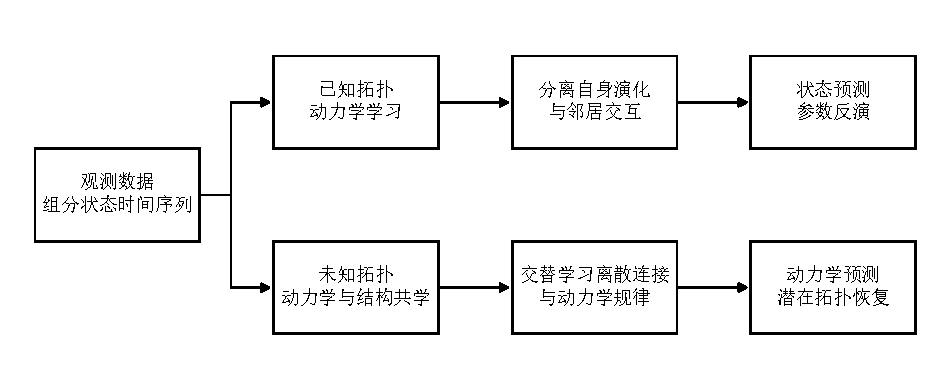
\includegraphics[width=\textwidth]{research_pipeline.pdf}
  \caption{本文研究路线。
相同的状态时间序列在网络已知与网络未知两种条件下形成递进任务：前者聚焦演化规律学习，后者进一步联合恢复潜在连接。
箭头仅表示信息与任务的推进关系。}
  \label{fig:pipeline}
\end{figure}

本文的主要工作包括以下三点。
\begin{enumerate}
  \item 提出一种面向网络动力学的自身--邻居双通道表示，将组分自身演化与邻居交互保持到读出阶段，以缓解量级失衡和表示混合，并通过多类图卷积对照分析其作用。
  \item 在网络不可见时，将离散拓扑生成与双通道动力学学习结合，通过硬图规律学习、软图结构更新和结构信息采样，构成从时间序列同时学习动力学与潜在网络的方法。
  \item 以 SIR 传播为可解释验证案例，从一步预测、参数反演、多步推演和边级恢复四个层面评价模型。
结果既展示了方法在三类网络上的有效性，
也揭示了联合学习仍可能出现的结构坍缩与适用边界。
\end{enumerate}

全文其余部分依次回顾数据驱动动力学学习、图神经网络与潜在关系推断的相关研究；
给出一般问题形式和 SIR 验证场景；
介绍已知与未知网络下的两阶段方法；
讨论实验结果、方法适用范围及向其他复杂系统动力学扩展的方向。

% !TEX root = ../main.tex
\section{相关工作}

\subsection{复杂网络与网络动力学}

复杂网络研究关注连接结构如何影响系统的集体行为。
随机网络、小世界网络和无标度网络分别提供了均匀随机连接、局部聚集与短路径并存、度分布高度异质等典型结构\cite{erdos1959,watts1998,barabasi1999}。
在这些网络上，
节点状态并非独立变化，
而是由自身规律和局部耦合共同驱动；
相同的节点动力学置于不同拓扑上，
可能呈现不同的传播阈值、同步模式和稳定性\cite{strogatz2001,albert2002}。

网络 SIR 是研究“结构如何塑造演化”的经典模型。
相较于均匀混合假设，网络模型把传播限定在连接边上，因此能够表达聚类、枢纽节点和局部暴发等效应\cite{pastorsatorras2015}。
本文使用 ER、WS 和 BA 网络并非为了把三者当作现实系统的替代，
而是希望在连接均匀性、局部聚集性和度异质性明显不同的条件下检验学习方法。

\subsection{数据驱动动力学学习}

数据驱动的动力学发现试图从观测轨迹中恢复状态演化规律。
稀疏辨识等方法通过预设函数库寻找简洁方程，为“从数据到规律”提供了重要思路\cite{brunton2016}；
神经网络方法则以更强的函数逼近能力处理难以事先列举的非线性关系。
对网络化系统而言，
核心并不是简单地把所有节点状态拼接为一个高维输入，
而是利用交互的局部性和共享性：每个节点遵循相似的更新形式，
但接收到的邻居作用由网络决定。

图神经网络恰好为这类关系提供了自然表示。
图卷积和 GraphSAGE 等方法通过聚合邻居信息完成节点级预测\cite{kipf2017gcn,hamilton2017}；
GIN 的分析进一步说明，
聚合函数能否保留邻居多重集合信息会影响模型的区分能力\cite{xu2019gin}。
本文使用的 GraphConv 基线对自身项与邻居项分别变换后相加\cite{morris2019,fey2019}。
在此基础上，
我们进一步保持两类表示的分离，
使模型可以独立调整自身演化和交互作用，
而不是把双通道优势归结为基线在结构上的“必然不可区分”。

\subsection{潜在关系学习与网络重构}

当拓扑不可见时，动力学学习还要回答“谁与谁发生作用”。
Neural Relational Inference 从多主体轨迹推断离散关系类型\cite{kipf2018nri}；
Gumbel Graph Network（GGN）则将网络生成器与动力学学习器联合训练，
以离散关系的连续松弛实现端到端优化\cite{zhang2019ggn}。
Gumbel-Softmax 和 Concrete 分布为这类离散采样提供了可微近似\cite{jang2017,maddison2017}。

联合学习的关键风险在于结构与动力学互相补偿：错误连接不一定立即造成较大预测误差，灵活的动力学模型可能通过改变交互强度吸收结构偏差。
本文沿用“生成网络并用预测误差反向约束结构”的基本思想，
但将第一阶段得到的双通道表示引入未知拓扑任务，
同时在硬图上学习规律，
并让结构更新使用软图梯度。
研究重点因此不是单纯提高一步预测精度，
而是在预测、规律诊断和边级恢复之间建立相互校验。

\subsection{本文研究定位}

已有研究分别提供了数据驱动方程发现、图表示学习和潜在关系推断的基础。
本文将这些线索组织为一个递进问题：先在网络已知时弄清怎样学习可解释、可推演的局部演化规律，
再在网络未知时处理规律与结构的共同辨识。
SIR 是本文用于验证这一路径的具体动力学，
而非方法成立的唯一对象。
方法所依赖的更一般假设是：组分状态可观测，
系统在给定时间尺度上近似满足局部马尔可夫更新，
交互能够由邻居状态的某种聚合表示。

% !TEX root = ../main.tex
\section{问题定义与实验设计}

\subsection{一般网络动力学问题}

设复杂系统包含 $N$ 个可观测组分，连接关系由邻接矩阵 $A$ 描述，全部组分在时刻 $t$ 的状态记为 $\mathbf X(t)=[\mathbf x_1(t),\ldots,\mathbf x_N(t)]$。
离散时间网络动力学可以一般地写为
\begin{equation}
\mathbf X(t+1)=\mathcal F_{\theta}\!\left(\mathbf X(t),A\right)+\boldsymbol\varepsilon(t),
\label{eq:network-dynamics}
\end{equation}
其中 $\mathcal F_{\theta}$ 表示未知或部分未知的演化规律，$\boldsymbol\varepsilon$ 概括过程随机性与观测误差。
若相互作用具有局部性和共享性，
节点更新还可写成
\begin{equation}
\mathbf x_i(t+1)\sim
f_{\theta}\!\left(
\mathbf x_i(t),+\operatorname{Agg}_{j:A_{ij}=1}
g_{\theta}(\mathbf x_i(t),\mathbf x_j(t))
\right).
\label{eq:local-interaction}
\end{equation}
这一表达将影响节点下一状态的因素分为两类：节点自身当前状态，以及由网络传入的邻居作用。
本文的方法围绕这一区分展开，而不要求 $f_{\theta}$ 具有某个特定动力学的解析形式。

据此定义两个递进任务。
网络已知时，给定 $A$ 和连续观测到的状态转移对，学习 $f_{\theta}$，并检验模型能否在未显式写入方程的情况下恢复正确的局部响应。
网络未知时，
只给出状态序列，
同时估计动力学参数 $\theta$ 与潜在邻接矩阵 $\hat A$。
第二项任务不仅要求预测准确，
还要求输出的连接能够在边级评价中接近真实网络。

\subsection{网络 SIR 动力学}

本文用离散时间网络 SIR 过程具体化\cref{eq:network-dynamics}。
在无向无自环网络上，节点 $i$ 的状态 $s_i(t)\in\{S,I,R\}$ 分别表示易感、感染和康复。
感染节点以概率 $\gamma$ 康复；
易感节点受到其感染邻居的独立影响。
时刻 $t$ 的感染者邻居数为
\begin{equation}
k_i(t)=\sum_j A_{ij}\,\mathbf{1}[s_j(t)=I],
\end{equation}
其中，$\mathbf{1}[\cdot]$ 为示性函数：方括号内的条件成立时取 1，否则取 0。
因此，$\mathbf{1}[s_j(t)=I]$ 仅在节点 $j$ 处于感染态时取 1，
与邻接矩阵元素 $A_{ij}$ 相乘并求和后，即得到节点 $i$ 的感染者邻居数。
相应的一步感染概率为
\begin{equation}
P(S\to I\mid k_i)=1-(1-\beta)^{k_i},
\label{eq:sir-infection}
\end{equation}
其中 $\beta$ 是单条感染边上的传播概率。
SIR 对本文尤其合适：一方面，节点自身状态决定可发生的转移，邻居计数决定交互强度，
与双通道思想直接对应；
另一方面，
\cref{eq:sir-infection}给出了可检验的真实响应曲线，
使“预测看起来正确”与“动力学规律确实被恢复”能够被区分。

\subsection{实验设计}

实验使用三类具有代表性的合成网络：ER 随机网络、WS 小世界网络和 BA 无标度网络。
每类只生成一个固定的 $N=100$ 图实例，
统一设置 $\beta=0.3$、$\gamma=0.1$。
对多组初始感染节点和随机传播轨迹进行模拟，
最终得到 9000 个相邻时刻状态转移对。
主要设置见\cref{tab:protocol}。

\begin{table}[H]
  \centering
  \caption{SIR 验证场景的数据与评价设置}
  \label{tab:protocol}
  \begin{tabularx}{0.96\textwidth}{@{}lX@{}}
    \toprule
    项目 & 设置 \\
    \midrule
    网络 & ER$(N=100,p=0.1)$、WS$(N=100,k=6,p=0.2)$、BA$(N=100,m=3)$，各一个固定实例 \\
    动力学 & 离散同步 SIR，$\beta=0.3$，$\gamma=0.1$，每条轨迹 60 个状态转移 \\
    观测数据 & 30 次初始节点抽样，每次模拟 5 条随机轨迹，共 9000 个状态转移对 \\
    数据划分 & 状态转移对按 $8:2$ 随机划分为训练集和验证集 \\
    规律诊断 & 感染概率随邻居数 $k$ 的变化、$\beta$ 与 $\gamma$ 的参数反演 \\
    多步推演 & 5 组初始条件、1--5 个初始感染者，比较 S/I/R 占比轨迹 \\
    结构评价 & 硬图的 ACC、Precision、F1、TPR、FPR 及预测边数 \\
    \bottomrule
  \end{tabularx}
\end{table}

评价遵循由“预测”到“规律”再到“结构”的层次。
一步预测使用逐节点交叉熵与准确率；
规律诊断比较模型给出的 $P(S\to I\mid k)$ 与理论曲线，
并从输出曲线反演 $\hat\beta$，
同时考察 $P(I\to R)$ 得到的 $\hat\gamma$；
多步推演把模型输出重新作为下一步输入，
统计群体 S/I/R 占比的平均绝对误差。
未知网络还使用
\begin{equation}
\mathrm{Precision}=\frac{TP}{TP+FP},\qquad
F_1=\frac{2\,\mathrm{Precision}\,\mathrm{TPR}}
{\mathrm{Precision}+\mathrm{TPR}}
\end{equation}
评价恢复的具体边，避免仅由大量真负边造成的高 ACC 掩盖稠密错误图。

多次训练采用同一图和同一数据上的不同优化初始化。
具体训练配置、结果文件与指标计算方式统一列于附录。

% !TEX root = ../main.tex
\section{已知拓扑下的动力学学习}

\subsection{局部交互表示}

当网络已知时，问题看似只是从 $\mathbf X(t)$ 预测 $\mathbf X(t+1)$，但真正关心的是模型能否形成可复用的局部更新规律。
对许多网络动力学而言，
节点变化都可以理解为两部分共同作用：一部分来自节点自身的状态和内在演化，
另一部分来自邻居传入的交互。
若模型把两者过早压入同一表示，
它可能依靠训练数据中的相关性获得不错的短期预测，
却在节点度数、网络类型或初始条件变化时产生不稳定响应。

SIR 案例把这一问题表现得十分清楚。
感染节点能否康复主要取决于自身状态，易感节点能否感染则取决于感染者邻居的绝对数量。
使用邻居均值时，
模型更容易看到感染邻居的比例，
而非数量；
在不同度数节点上，
相同的比例可能对应完全不同的感染风险。
因此本文使用求和聚合保存交互数量，
并把均值聚合作为对照。

\subsection{融合式基线与双通道表示}

本文的 GraphConv 基线并不是把自身和邻居原始特征直接相加。
其一层更新为
\begin{equation}
\mathbf h_i^{(\ell+1)}=\sigma\!\left(
W_{\mathrm{self}}^{(\ell)}\mathbf h_i^{(\ell)}
+W_{\mathrm{neigh}}^{(\ell)}
\sum_{j\in\mathcal N(i)}\mathbf h_j^{(\ell)}
\right),
\label{eq:graphconv}
\end{equation}
即先对自身项和邻居项分别变换，再在隐藏空间相加。
它具有表达不同作用的能力，但相加之后两类贡献不再分别可见；
当节点度数增大时，邻居求和的幅度还可能明显超过自身项，
形成量级失衡和表示干扰。

为此，本文采用自身--邻居双通道结构：
\begin{align}
\mathbf z_i^{\mathrm{self}}&=f_{\mathrm{self}}(\mathbf x_i),\\
\mathbf z_i^{\mathrm{neigh}}&=
f_{\mathrm{neigh}}\!\left(\sum_{j\in\mathcal N(i)}g(\mathbf x_j)\right),\\
\hat{\mathbf y}_i&=f_{\mathrm{out}}\!
\left([\mathbf z_i^{\mathrm{self}};\mathbf z_i^{\mathrm{neigh}}]\right).
\end{align}
如\cref{fig:architecture}所示，两类信息直到读出阶段才合并。
该设计并不预设 SIR 的感染概率公式，只规定模型以“自身演化 + 邻居作用”的方式组织信息。
因此，
它同样可用于其他满足局部交互假设的网络动力学；
对于不同任务，
邻居通道中的求和也可替换为加权聚合、注意力或其他与物理交互相符的算子。

\begin{figure}[H]
  \centering
  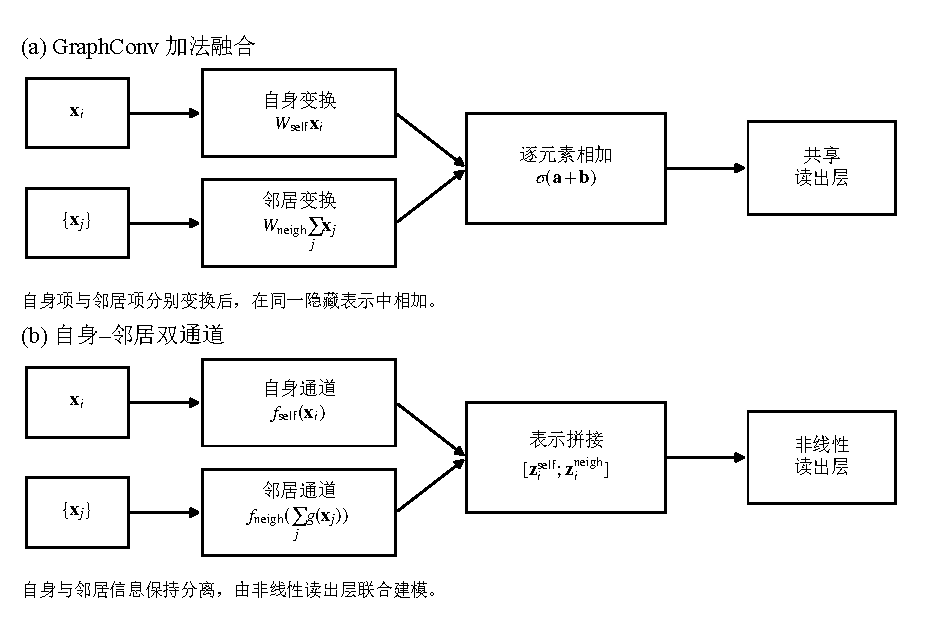
\includegraphics[width=\textwidth]{architecture_compare.pdf}
  \caption{融合式 GraphConv 基线与自身--邻居双通道模型。
(a) 基线对自身项和邻居项分别变换后相加；
(b) 双通道将自身演化与邻居交互保持到读出阶段，
从而缓解量级失衡和表示混合。}
  \label{fig:architecture}
\end{figure}

\subsection{对照模型与评价设计}

为理解表示选择带来的影响，已知网络实验比较五个模型：单向求和 GraphConv、双向求和 GraphConv、增加隐藏非线性的双向求和 GraphConv、双向均值 GraphConv以及双向双通道模型。
这里的“单向”并非一种合理的无向网络模型，
而是边表未显式补齐反向消息时的实现缺陷对照；
它用于说明网络数据进入消息传递框架时，
边方向处理同样会影响所学规律。

比较并不只看一步分类结果。
感染概率随邻居数变化的曲线用于判断模型是否学到了正确的交互响应，参数反演用于概括曲线与真实机制的接近程度，
多步自回归则检验小的一步偏差是否会在闭环中累积。
这样的多层评价能够区分两类模型：一种只是对当前样本分类较准，
另一种同时保留了可解释且可推演的动力学关系。
具体层数、训练轮数和优化参数列于附录。

% !TEX root = ../main.tex
\section{未知拓扑下的动力学与拓扑联合学习}

\subsection{动力学与结构联合辨识}

移除已知网络之后，模型必须同时回答两个彼此关联的问题：怎样的局部规律能够解释观测到的状态变化，哪些节点之间存在足以支持这种解释的连接。
直观上，
真正相互作用的节点应当在时间序列中留下稳定的条件依赖；
但由于状态变化具有随机性，
而且动力学学习器具有较强的函数逼近能力，
错误结构也可能被参数调整暂时掩盖。

本文把这种现象称为结构--动力学补偿。
例如，生成器给出过多邻居时，学习器可以减小单个邻居的平均作用，使总输入仍落在合理范围内。
这样得到的模型可能具有较低的一步损失，
却不能提供可信的连接解释。
未知网络任务因此不能只是“把邻接矩阵也设成参数”，
还需要限制结构与规律相互替代的自由度。

\subsection{可学习的离散拓扑}

本文为每个无序节点对维护一个可训练的连接倾向 $R_{ij}$，并通过 Gumbel--Softmax 和 Concrete 松弛产生可微的软邻接矩阵\cite{jang2017,maddison2017}：
\begin{equation}
\hat A_{ij}^{\mathrm{soft}}
=\sigma\!\left(\frac{R_{ij}+G_{ij}}{\tau}\right),
\qquad G_{ij}\sim\operatorname{Logistic}(0,1).
\label{eq:gumbel-soft}
\end{equation}
上三角变量被镜像到下三角，对角线固定为零，从而保证候选图无向且无自环。
需要输出具体网络时，使用 0.5 阈值得到硬连接
\begin{equation}
\hat A_{ij}^{\mathrm{hard}}=\mathbf{1}[R_{ij}+G_{ij}>0].
\label{eq:hard-sample}
\end{equation}
当连接倾向与采样噪声之和 $R_{ij}+G_{ij}>0$ 时，节点 $i$ 与 $j$ 之间保留一条边；
否则不保留该边。
温度 $\tau$ 改变软图的锐度与反向传播梯度，但在给定 $R_{ij}$ 和噪声时，并不直接改变 0.5 阈值下的硬采样结果。

生成的候选网络进入双通道动力学学习器。
自身通道仍描述节点内在变化，邻居通道则通过 $\hat A\,g(\mathbf X)$ 汇聚候选邻居的作用。
这样，
已知网络阶段形成的表示原则可以直接延伸到潜在网络：区别仅在于交互对象不再预先给出，
而要由观测数据共同确定。

\subsection{硬图规律学习与软图结构更新}

联合训练采用交替策略，如\cref{fig:joint-flow}所示。
在动力学学习阶段，从当前连接分布采样一张离散硬图，固定该图并更新双通道学习器。
由于每条边只能取 0 或 1，
学习器不能简单地把大量多余边都缩成很小的连续权重。
在结构更新阶段，
冻结学习器，
使用软图计算预测误差并把梯度传回连接倾向；
熵正则促使边概率远离难以解释的中间值。

\begin{figure}[H]
  \centering
  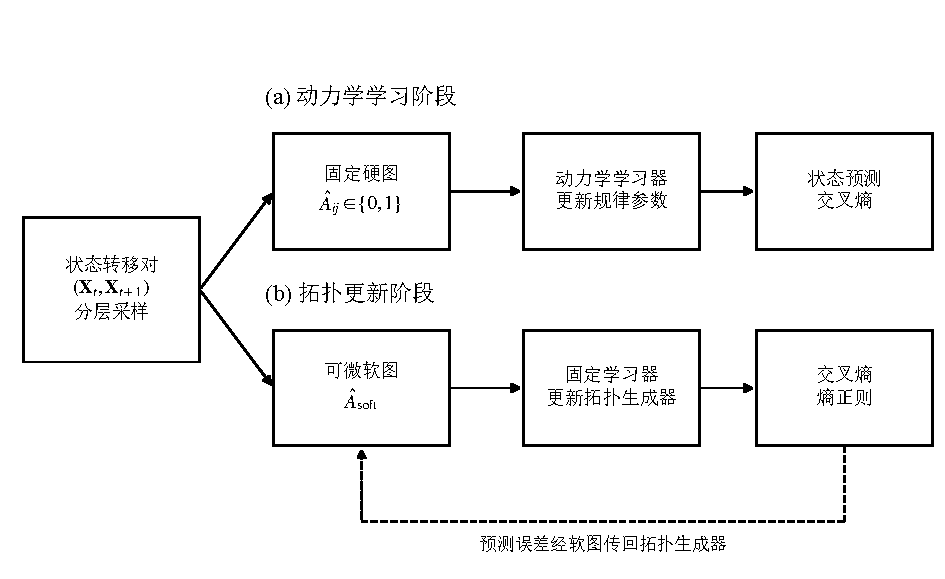
\includegraphics[width=\textwidth]{joint_training_flow.pdf}
  \caption{动力学与拓扑的交替学习。
硬图阶段更新演化规律，软图阶段利用可微松弛更新连接倾向；
两者共享同一预测目标，但承担不同的学习角色。}
  \label{fig:joint-flow}
\end{figure}

硬图学习削弱了连续弱边补偿。
本文进一步结合数据组织和模型选择，使连接辨识得到更充分的观测证据与验证信号。

\subsection{结构信息引导的分层采样}

传播轨迹中常有大量接近吸收态的时刻：系统中已经没有感染节点，或绝大多数节点只保持原状态。
这些样本有助于学习状态保持，却几乎不提供“影响沿哪条边传递”的信息。
如果训练始终被这类样本主导，
模型便可能在缺少结构证据的情况下优化出较低损失。

为此，本文按照每个时刻的感染节点数量分层，并在各层中无放回抽样，使低、中、高传播活动状态都能稳定进入每轮训练。
该设计在 SIR 中以感染者数量实现；
推广到其他动力学时，
可替换为状态变化幅度、活跃组分数量或局部事件强度等任务相关指标。
验证集仍保持原始分布，
避免选模只偏向重采样后的训练分布。

每类网络从三个不同初始化开始联合学习，最终只根据验证交叉熵选择一个模型，不使用真实边进行选模。
多初始化扩大了候选解的搜索范围，验证损失提供统一的选择依据。
完整的采样配额、训练节奏和九次运行结果均置于附录。

% !TEX root = ../main.tex
\section{实验结果与分析}

\subsection{已知拓扑下的动力学学习性能}

首先考察网络已知时，模型能否从状态转移数据中恢复 SIR 的局部演化关系。
\cref{tab:known-main}给出五个模型在 ER、WS 和 BA 三类网络上的平均结果。
双向双通道模型的感染率反演误差、完整感染曲线误差、恢复率误差和自回归误差均为五者最低。
这组结果体现了双通道模型在预测、规律校准和多步推演之间的综合优势。

\begin{table}[H]
  \centering
  \caption{已知网络时五类学习器在 ER、WS、BA 上的平均结果}
  \label{tab:known-main}
  \begin{threeparttable}
  \begin{tabular}{@{}lccccc@{}}
    \toprule
    模型 & $|\hat\beta-0.3|$ & 逐 $k$ MAE & $|\hat\gamma-0.1|$ & $\Delta\gamma$ & 自回归 MAE(I) \\
    \midrule
    单向求和 GraphConv-1L & 0.09089 & 0.19924 & 0.00297 & 0.00719 & 0.03693 \\
    双向求和 GraphConv-1L & 0.07940 & 0.09188 & 0.00877 & 0.03437 & 0.03219 \\
    双向求和 GraphConv-3L & 0.02356 & 0.02730 & 0.00602 & 0.01039 & 0.01134 \\
    双向均值 GraphConv-3L & 0.02355 & 0.13654 & 0.00472 & \textbf{0.00050} & 0.01386 \\
    {\yahei 双向双通道} & \textbf{0.00406} & \textbf{0.01296} & \textbf{0.00234} & 0.00135 & \textbf{0.00789} \\
    \bottomrule
  \end{tabular}
  \end{threeparttable}
\end{table}

\cref{fig:known-results}进一步揭示了差异从何而来。
BA 网络包含少量高度数节点，最容易暴露聚合方式的问题。
均值聚合在中高邻居数区域给出的感染概率趋于平台，
说明感染邻居比例不能稳定替代绝对数量；
单向边表因遗漏部分消息而产生更明显偏差。
增加隐藏非线性后，
求和 GraphConv 已能恢复曲线的大致形状，
但双通道模型在不同节点度数上的响应更一致。
这说明分离表示能够减轻量级失衡和信息混合，
使局部交互响应更加稳定。

\begin{figure}[!htbp]
  \centering
  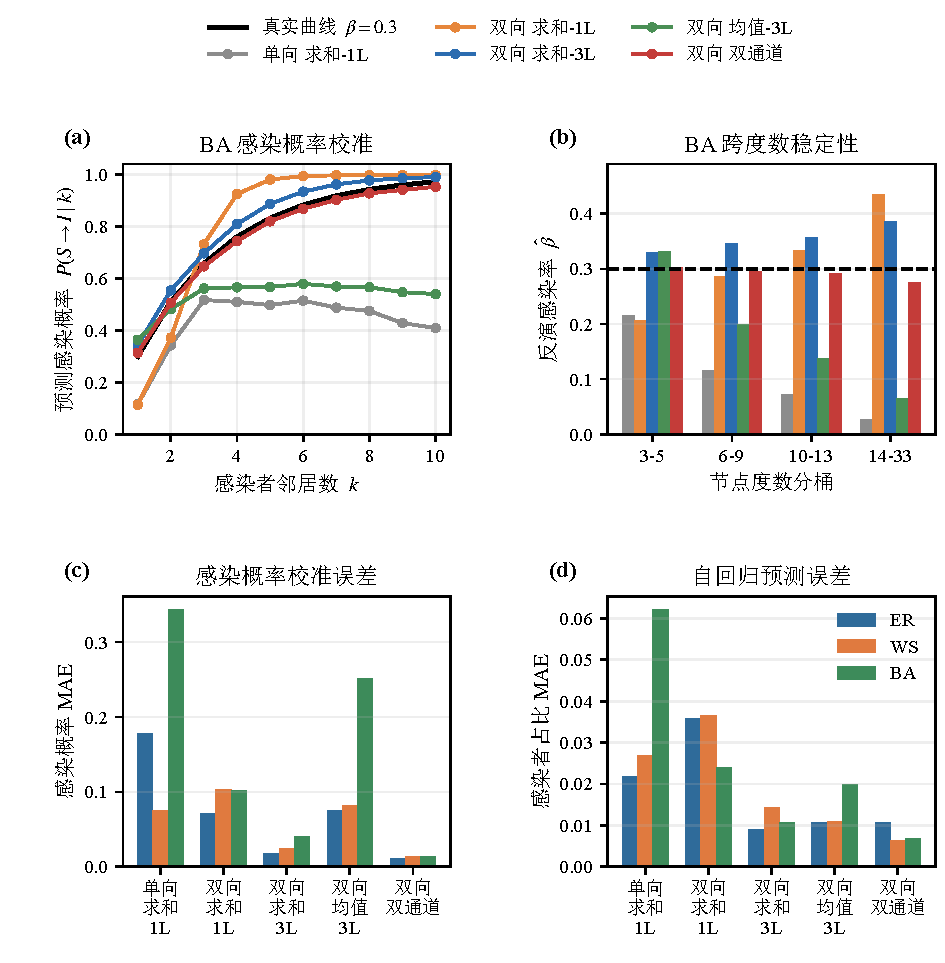
\includegraphics[width=\textwidth]{known_topology_results.pdf}
  \caption{已知网络时五类学习器的比较。
(a) BA 网络的感染概率曲线；
(b) BA 网络按节点度数得到的感染率反演；
(c) 三类网络的曲线误差；
(d) 三类网络的多步推演误差。}
  \label{fig:known-results}
\end{figure}

双通道模型在 ER、WS、BA 上反演得到的 $\hat\beta$ 分别为 0.3036、0.3079 和 0.3007，与真实值 0.3 接近；
逐 $k$ 误差分别为 0.0111、0.0137 和 0.0140。
其感染者占比自回归 MAE 分别为 0.0106、0.0063 和 0.0067，
表明一步规律在闭环推演中没有快速偏离。
三个网络上的感染响应与群体演化结果共同支持了分离表示对动力学学习的积极作用。

\subsection{未知拓扑下的网络重构性能}

进一步移除真实网络，只保留状态时间序列。
按照验证交叉熵选择的三个模型见\cref{tab:unknown-main}。
在该组固定实例上，
WS 网络被完整恢复；
BA 只多预测 4 条边；
ER 存在 41 条假阳性边和 24 条假阴性边，
但硬图 F1 仍达到 0.9374。
三类网络的 Precision 和 F1 均明显高于仅靠预测稠密网络可能得到的水平，
说明模型恢复的不只是能够参与计算的任意权重矩阵，
而是与真实连接高度一致的离散图。

\begin{table}[H]
  \centering
  \caption{未知网络时所选模型的拓扑恢复、参数诊断与多步推演结果}
  \label{tab:unknown-main}
  \resizebox{\textwidth}{!}{%
  \begin{tabular}{@{}lccccccccccc@{}}
    \toprule
    网络 & seed & 验证 CE & ACC & Precision & F1 & TPR & FPR & 边数 & $\hat\beta$ & $\hat\gamma\pm s$ & MAE(I) \\
    \midrule
    ER & 42 & 0.073868 & 0.9869 & 0.9223 & 0.9374 & 0.9530 & 0.0092 & 528/511 & 0.2942 & $0.1039\pm0.0028$ & 0.0072 \\
    WS & 7  & 0.074515 & 1.0000 & 1.0000 & 1.0000 & 1.0000 & 0.0000 & 300/300 & 0.2996 & $0.1008\pm0.0028$ & 0.0059 \\
    BA & 7  & 0.074649 & 0.9992 & 0.9864 & 0.9932 & 1.0000 & 0.0009 & 295/291 & 0.2889 & $0.1037\pm0.0022$ & 0.0082 \\
    \bottomrule
  \end{tabular}}
  \parbox{\textwidth}{\footnotesize\vspace{0.35em}注：$s$ 表示不同控制状态上模型输出的离散程度，
不是统计置信区间。}
\end{table}

\cref{fig:seed-recon}(a)展示全部九次优化及最低验证交叉熵选出的模型。
三个网络上，所选结果均位于较低验证损失与较高硬图 F1 的区域，
表明验证信号在本组实验中能够有效识别高质量候选网络。
图中同时保留其他初始化结果，
便于观察选模过程；
不同优化结果的差异及其机制在讨论部分分析。

\begin{figure}[!htbp]
  \centering
  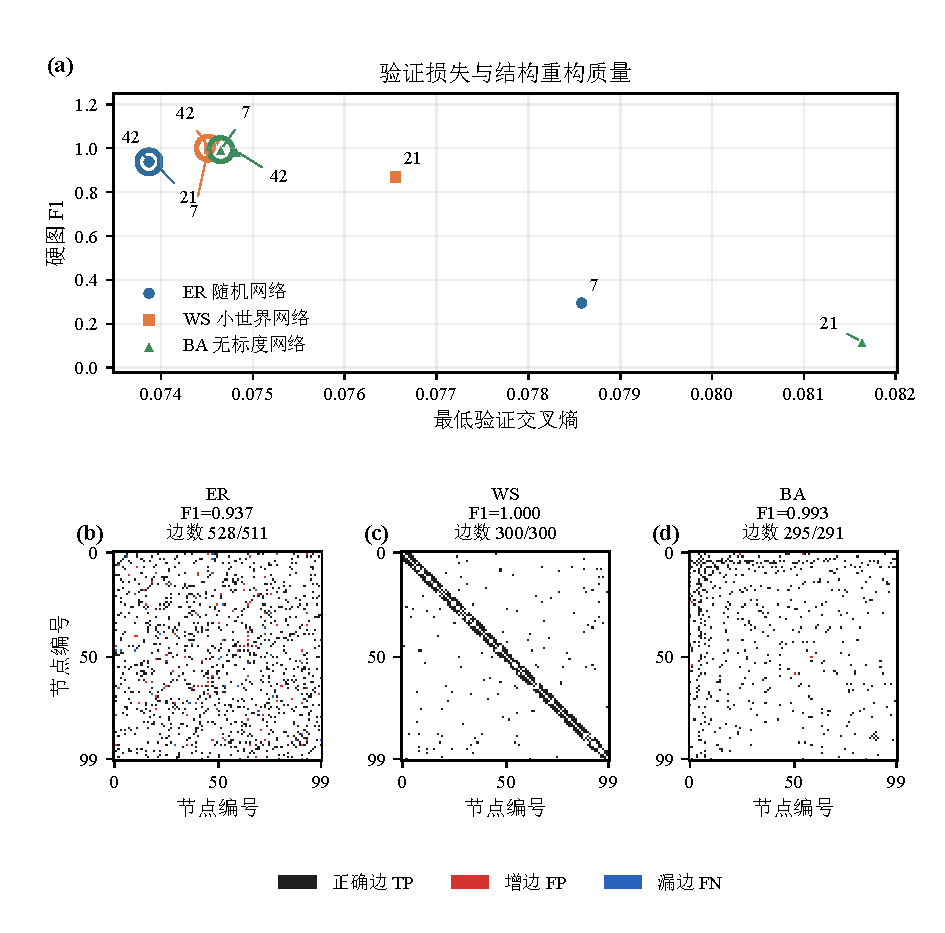
\includegraphics[width=\textwidth]{seed_selection_and_reconstruction.pdf}
  \caption{不同初始化与拓扑恢复结果。
(a) 九次训练的验证交叉熵和硬图 F1，数字为训练 seed，空心圆为所选模型；
(b)--(d) ER、WS、BA 所选硬图中的正确边、假阳性边和假阴性边。}
  \label{fig:seed-recon}
\end{figure}

软图 AUC 在三个所选模型上分别为 0.9863、1.0000 和 1.0000，但 AUC 只反映边分数的排序，不能说明固定阈值下会保留多少错误边。
本文因此把 Precision、F1 和预测边数作为结构结论的主要依据。
这一选择也体现了全文的基本判断：用于预测的连续关系分数与最终需要解释的离散网络并不是同一件事。

\subsection{参数反演与多步预测性能}

\cref{fig:calibration-autoreg}从参数诊断和多步推演两个层面展示重构网络对动力学预测的支持。
未知网络时，
ER、WS、BA 的感染率反演值分别为 0.2942、0.2996 和 0.2889，
恢复率反演值分别为 0.1039、0.1008 和 0.1037；
前者整体接近真实值 0.3，
后者接近真实值 0.1，
体现了所学局部响应与真实动力学的一致性。

\begin{figure}[!htbp]
  \centering
  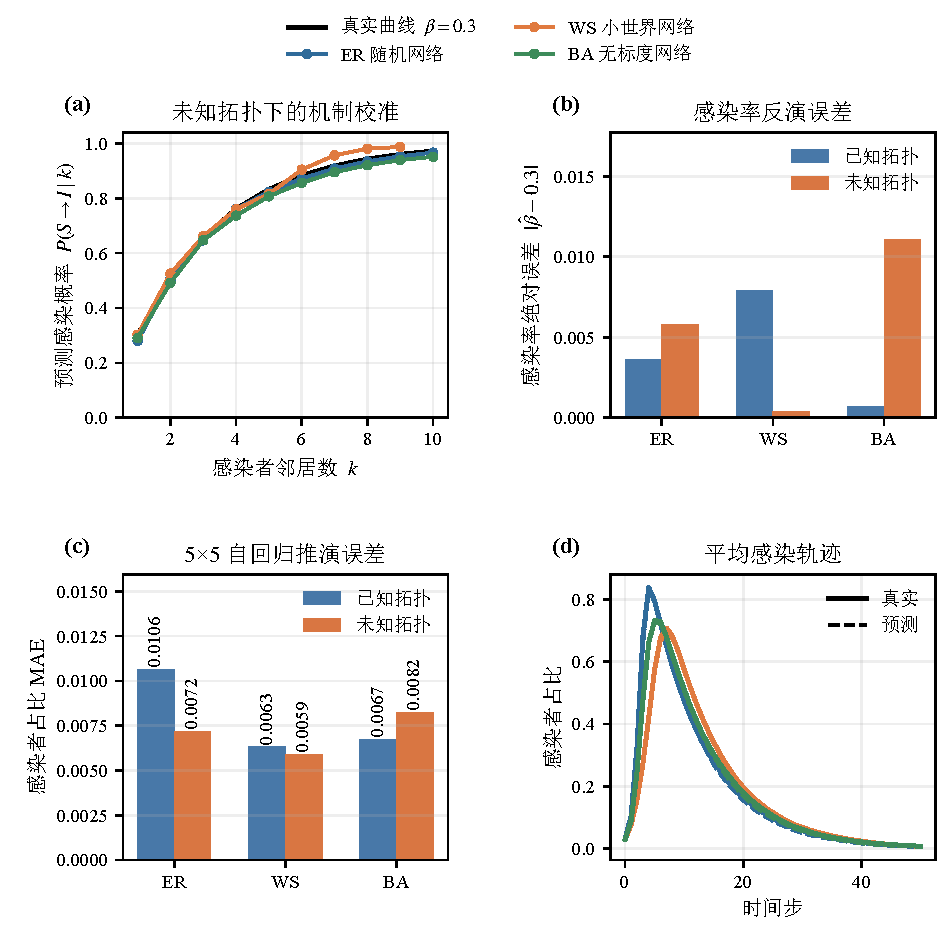
\includegraphics[width=\textwidth]{calibration_and_autoregression.pdf}
  \caption{规律诊断与多步推演。
(a) 未知网络时学习到的感染响应；
(b) 已知与未知网络下的感染率反演误差；
(c) 两阶段的感染者占比自回归误差；
(d) 未知网络模型在代表性初始条件下的平均感染者轨迹。
两阶段训练条件不同，
图中并列只用于比较误差量级。}
  \label{fig:calibration-autoreg}
\end{figure}

未知网络下三类模型的感染者占比自回归 MAE 为 0.00716、0.00588 和 0.00824，三状态平均 MAE 为 0.00609、0.00510 和 0.00886。
它们与已知网络双通道模型处在相近量级，
说明所恢复的连接能够支撑稳定的闭环演化，
而不仅是一次性的边集合匹配。
在本组实验条件下，
这些结果表明动力学规律与主要拓扑可以由同一组时间序列共同恢复。
\FloatBarrier

% !TEX root = ../main.tex
\section{讨论与展望}

\subsection{方法有效性与机制分析}

本文从一个具体的传播模型出发，但希望回答的是更一般的问题：当复杂系统只留下多变量时间序列时，如何把演化规律与交互结构重新分离出来。
SIR 的价值在于它足够简单，
使真实感染曲线、传播参数和网络边都可以被精确检查；
同时它又包含随机性、非线性交互和吸收态，
能够暴露普通分类指标不易发现的问题。

实验首先说明，准确的一步预测并不等同于可信的动力学学习。
均值聚合和单向边表在常见状态上仍能得到一定预测能力，却难以稳定恢复感染概率对邻居数量的响应。
把自身演化与邻居交互分开表示后，
模型在不同网络结构和多步推演中的校准更稳定。
这里真正可推广的不是“感染者邻居计数”本身，
而是根据系统机理区分内在动力与外部耦合，
并选择能够保留交互强度的聚合方式。

实验还说明，动力学预测与拓扑解释必须相互验证。
未知网络时，稠密错误图仍可能通过动力学参数补偿获得看似可接受的短期输出。
硬图训练减少了一类连续缩放补偿，
分层样本让更多结构事件进入训练，
多初始化则帮助避开部分局部解；
然而九次运行中的两次严重坍缩表明，
结构辨识并没有因这些设计而被彻底解决。

\subsection{方法的可扩展性}

双通道框架依赖的核心结构是\cref{eq:local-interaction}，而不是 SIR 的具体概率公式。
只要组分状态能够被观测，
节点更新可以近似拆分为自身演化与邻居作用，
方法就具有迁移潜力。
例如，
SIS、SEIR 等传播模型可以通过扩展节点状态实现；
观点演化和信息扩散可以把邻居通道改为带方向或带符号的影响；
耦合振子、生态网络和电力系统则需要把离散分类读出替换为连续状态预测，
并采用与相互作用形式相符的聚合算子。

这种推广并非简单更换数据集。
不同动力学中的“结构证据”并不相同：SIR 中是感染事件与活跃感染者数量，振荡系统中可能是相位差和同步破缺，
生态系统中可能是扰动后的协同变化。
网络也可能有方向、权重、符号和时间变化。
因而，
本文提供的是一个方法框架和一组设计原则，
而不是无需修改即可覆盖所有复杂系统的通用成品模型。

\subsection{方法局限与实验边界}

模型的综合优势需要结合各指标和实验条件理解。
已知拓扑实验中，均值聚合模型的平均 $\Delta\gamma=0.00050$ 小于双通道的 0.00135；
ER 上三层求和 GraphConv 的自回归 MAE 为 0.0090，
也略低于双通道的 0.0106。
因此，
跨网络综合性能优势并不意味着每项指标均最优。
未知拓扑模型对 BA 的感染率反演值为 0.2889，
仍存在约 0.011 的低估。

九次优化中，ER 随机种子 7 和 BA 随机种子 21 分别生成 2955 条和 4586 条预测边，F1 为 0.2949 和 0.1193；
WS 随机种子 21 将 300 条真实边扩张为 390 条。
最低验证交叉熵在本组实验中排除了严重稠密解，
但三个初始化不足以估计稳定的失败概率，
也不能保证对新网络具有同样的筛选效果。

此外，未知拓扑阶段使用 100 轮训练和三个初始化选模，已知拓扑阶段使用 30 轮训练和单个初始化。
两阶段结果适合比较误差量级，不构成严格匹配训练预算的性能排名；
现有对照也未完全隔离参数量、采样与优化设置的影响。

本文的实验边界还体现在以下方面。
\begin{enumerate}
  \item {\yahei 网络与参数范围有限。}ER、WS、BA 各只有一个 $N=100$ 固定实例，且只使用 $\beta=0.3,\gamma=0.1$。
当前结果支持实例级方法验证，
不能替代跨网络、跨参数的统计结论。
  \item {\yahei 观测条件理想化。}节点身份已对齐，状态同步、完整且无标签噪声，网络静态、无向、无自环。
现实数据中的漏报、异步采样、潜变量和时变连接都会增加辨识难度。
  \item {\yahei 泛化检验仍较弱。}训练与验证按状态转移对随机划分，同一轨迹的相邻时刻可能进入不同集合；
因此验证交叉熵主要衡量同分布拟合与选模，
而非对全新轨迹的严格外推。
  \item {\yahei 联合优化仍不稳定。}三个训练 seed 只能展示初始化敏感性，不能估计可靠的失败概率。
生成器还需要维护平方级数量的候选关系，
对大规模网络的计算和搜索压力较高。
\end{enumerate}

这些限制并不否定已观察到的结果，但决定了结论应如何表达：本文证明了在受控 SIR 场景中，由状态时间序列联合恢复规律与结构是可行的，并找到了影响稳定性的关键机制；
它尚未证明任何满足局部交互的系统都能被同样准确地重构。

\subsection{未来研究方向}

未来研究将围绕“其他理论模型上的验证”与“真实复杂系统中的验证和拓展”两个方向展开，
逐步检验本文方法在不同动力学机制与观测条件下的适用性。

第一，在其他网络动力学理论模型上开展受控验证。
以复杂网络上的 Kuramoto 模型等为代表，
将研究对象从离散传播状态拓展到连续动力学，
根据相应的局部相互作用形式调整邻居表示、聚合算子和预测读出。
在已知真实规律与拓扑的条件下，
考察模型能否同时恢复局部交互、重构网络连接并预测群体演化。
通过多网络实例、不同参数条件和轨迹级划分，
进一步辨析双通道表示与交替结构学习的共性优势及其适用边界。

第二，在真实复杂系统中验证并拓展该框架。
面向金融市场、电网系统等场景，
探索如何从实际观测时间序列中学习组分间的有效相互作用，
并将所学关系用于动态预测和系统行为分析。
针对真实数据中的噪声、缺失、非平稳性和潜在外部驱动，
结合领域知识扩展有向、加权或时变的关系表示，
通过样本外预测、结构稳定性以及可获得的外部信息检验模型。
尤其需要区分预测性的依赖关系与真实物理连接或因果作用，
避免把较高预测精度直接解释为结构辨识成功。

这两个方向相互补充：理论模型提供可核验的方法检验基础，
真实系统则推动观测处理、关系表示与评价方式的进一步完善。
最终目标是形成能够连接时间序列观测、动力学预测与网络结构解释的复杂系统学习方法。

% !TEX root = ../main.tex
\section{结论}

本文研究了一个面向复杂系统的基础逆问题：当可获得的信息主要是各组分的状态时间序列时，如何学习网络上的演化规律，并在连接关系不可见时进一步重构潜在拓扑。
围绕这一目标，
本文形成了由已知网络到未知网络的递进方法。
前者以自身--邻居双通道分别表示组分内在变化与局部交互，
后者在此基础上加入离散拓扑生成器，
通过硬图规律学习与软图结构更新交替优化。

网络 SIR 为这套方法提供了可解释的验证环境。
已知网络实验表明，分离表示能够缓解邻居累积量级与自身状态之间的干扰，在感染曲线、参数反演和多步推演上取得更稳定的综合结果。
未知网络实验进一步表明，
在 ER、WS 和 BA 三个固定实例上，
模型可以仅依据状态转移数据恢复 F1 为 0.937--1.000 的硬图，
并保持接近真实传播参数的演化响应和较低的自回归误差。

本文还建立了连接一步预测、规律诊断、多步推演和边级恢复的评价方式。
各层面结果相互印证，使模型性能既能以预测误差衡量，也能由局部机制和潜在连接的恢复加以解释，
为复杂系统的数据驱动建模提供了更完整的评价依据。

本文并不把 SIR 视为方法的边界。
自身演化与交互作用的分解、离散结构与动力学的联合约束，以及多层次评价原则，都具有迁移到其他网络动力学的潜力。
未来将通过更多动力学类型、独立网络实例、噪声和缺失观测以及有向、加权和时变网络，
系统检验这一潜力，
并推动方法由受控验证走向真实复杂系统的建模与预测。


\clearpage
\printbibliography[title={参考文献}]

\clearpage
\appendix
% !TEX root = ../main.tex
\section{实验配置与完整结果}

\subsection{主要训练超参数}

表\ref{tab:hyperparams}给出两个阶段的主要超参数。
已知与未知拓扑阶段的训练预算明显不同，因此正文只比较误差量级，
不进行严格的阶段间性能排名。

\begin{table}[H]
  \centering
  \caption{已知拓扑 phase4 与未知拓扑 phase6 的主要训练配置。}
  \label{tab:hyperparams}
  \begin{tabularx}{0.95\textwidth}{@{}l>{\raggedright\arraybackslash}X>{\raggedright\arraybackslash}X@{}}
    \toprule
    配置 & 已知拓扑 phase4 & 未知拓扑 phase6 \\
    \midrule
    训练轮数 & 30 & 100 \\
    隐藏维数 & 64 & 64 \\
    批量大小 & 32 & 64 \\
    学习率 & 0.01 & 学习器 0.001；生成器 0.05 \\
    优化器 & Adam & Adam \\
    dropout & 0.2 & 未使用 \\
    训练 seed & 21 & 7、21、42 \\
    数据 seed & 21 & 21（固定缓存） \\
    温度 & 不适用 & 指数退火 3.0 $\to$ 0.1 \\
    每轮学习器更新 & 全训练集 1 轮 & 固定硬图，全训练集 3 轮 \\
    每轮生成器更新 & 不适用 & 软图 20 批 \\
    正则 & 无 & 熵正则 $\lambda=0.005$ \\
    样本策略 & 原始训练集 & 四层无放回配额 300/2700/1800/1200 \\
    \bottomrule
  \end{tabularx}
\end{table}

\subsection{未知拓扑全部训练随机种子}

表\ref{tab:all-seeds}列出 9 次结构学习运行。
最低验证 CE 规则选中 ER seed 42、WS seed 7 和 BA seed 7。
ER seed 7 与 BA seed 21 的 TPR 均为 1，
但 Precision 很低，
说明模型几乎把所有真实边包含在一个严重过密的预测图中；
只报告 TPR 会掩盖这一失败模式。

\begin{table}[H]
  \centering
  \caption{未知拓扑阶段全部 9 次运行。
星号表示该网络最终选中的 seed。}
  \label{tab:all-seeds}
  \begin{tabular}{@{}lrrrrrrr@{}}
    \toprule
    网络 & seed & 验证 CE & ACC & Precision & F1 & TPR & 预测/真实边数 \\
    \midrule
    ER & 7  & 0.078580 & 0.5063 & 0.1729 & 0.2949 & 1.0000 & 2955/511 \\
    ER & 21 & 0.073931 & 0.9851 & 0.9009 & 0.9299 & 0.9609 & 545/511 \\
    ER & 42$^*$ & 0.073868 & 0.9869 & 0.9223 & 0.9374 & 0.9530 & 528/511 \\
    WS & 7$^*$ & 0.074515 & 1.0000 & 1.0000 & 1.0000 & 1.0000 & 300/300 \\
    WS & 21 & 0.076552 & 0.9818 & 0.7692 & 0.8696 & 1.0000 & 390/300 \\
    WS & 42 & 0.074528 & 0.9998 & 0.9967 & 0.9983 & 1.0000 & 301/300 \\
    BA & 7$^*$ & 0.074649 & 0.9992 & 0.9864 & 0.9932 & 1.0000 & 295/291 \\
    BA & 21 & 0.081632 & 0.1323 & 0.0635 & 0.1193 & 1.0000 & 4586/291 \\
    BA & 42 & 0.074818 & 0.9984 & 0.9764 & 0.9864 & 0.9966 & 297/291 \\
    \bottomrule
  \end{tabular}
\end{table}

\subsection{已知拓扑完整六面板诊断}

图\ref{fig:appendix-known-overview}给出 ER、WS、BA 三类网络的完整六面板诊断，用于核查正文压缩图中未展开的分桶恢复率、$\Delta\gamma$ 和初始感染人数敏感性。
由于每张图信息密度较高，
统一置于横向附录页。

\begin{landscape}
\begin{figure}[p]
  \centering
  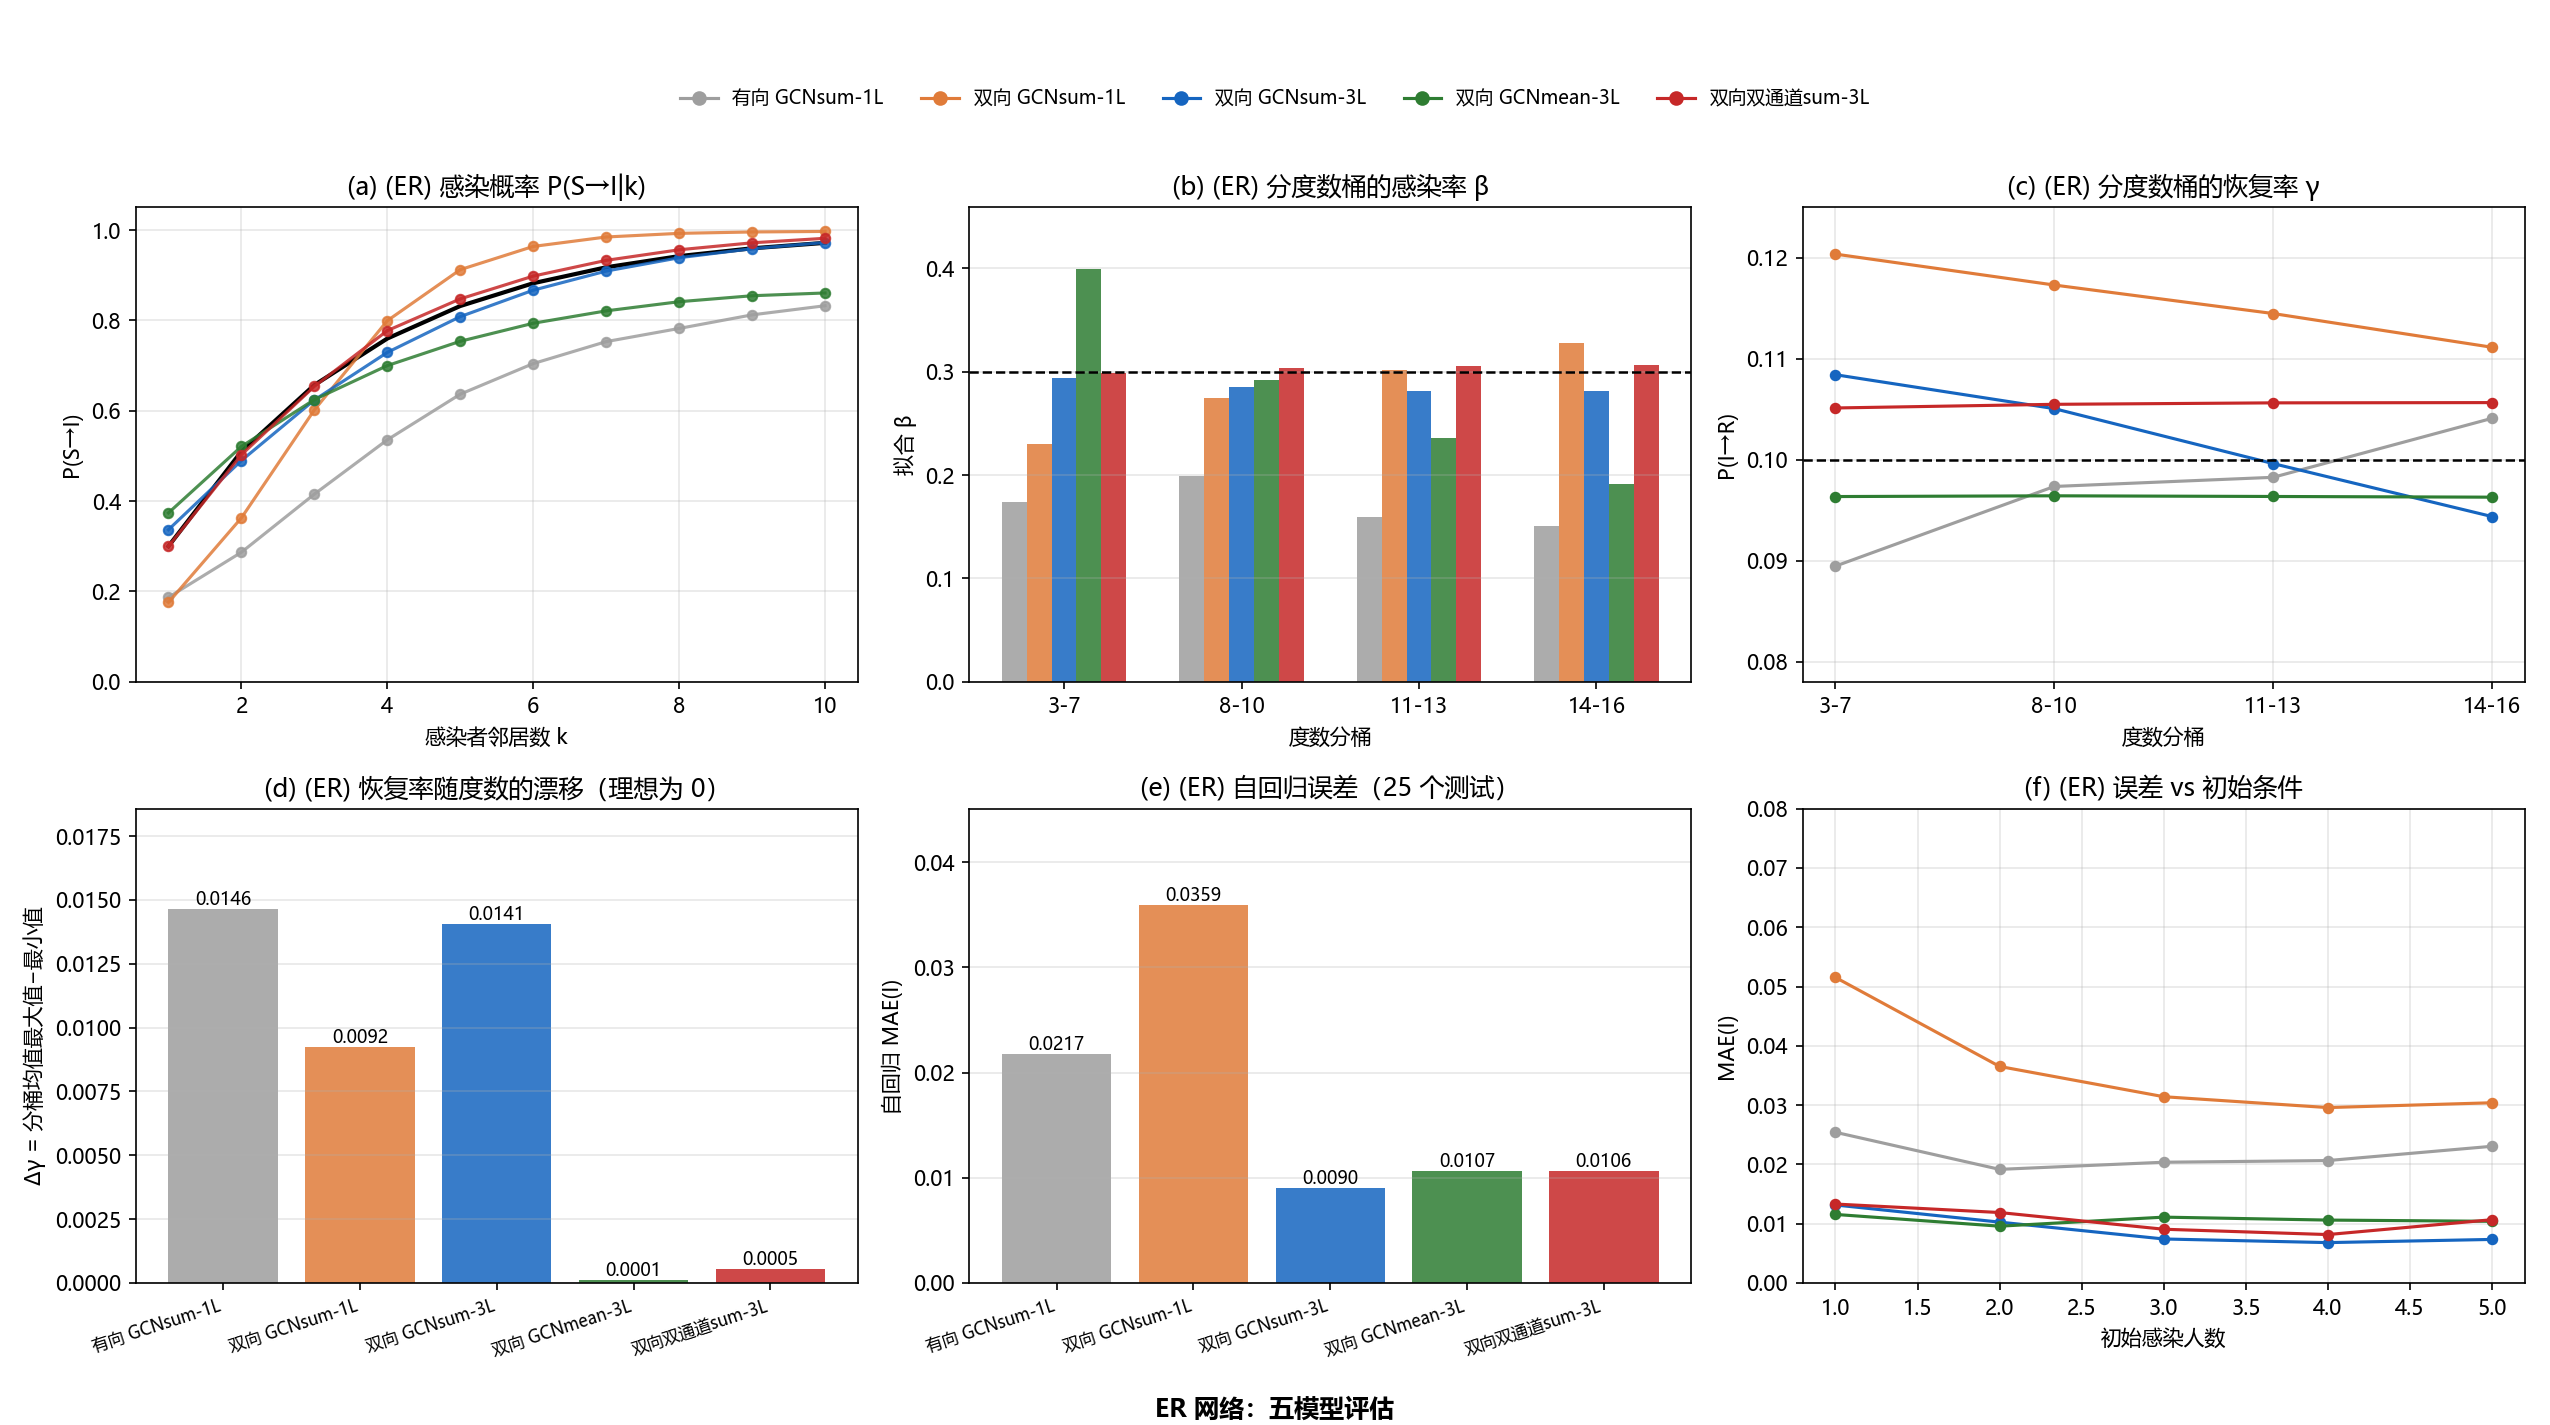
\includegraphics[width=0.96\linewidth]{fig_overview_ER.png}
  \caption{已知拓扑：ER 网络五模型完整诊断。
图中模型名称沿用 phase4 结果文件；
正文将 \code{twob3l\_bi} 统一称为双向双通道模型。}
  \label{fig:appendix-known-overview}
\end{figure}
\end{landscape}

\begin{landscape}
\begin{figure}[p]
  \centering
  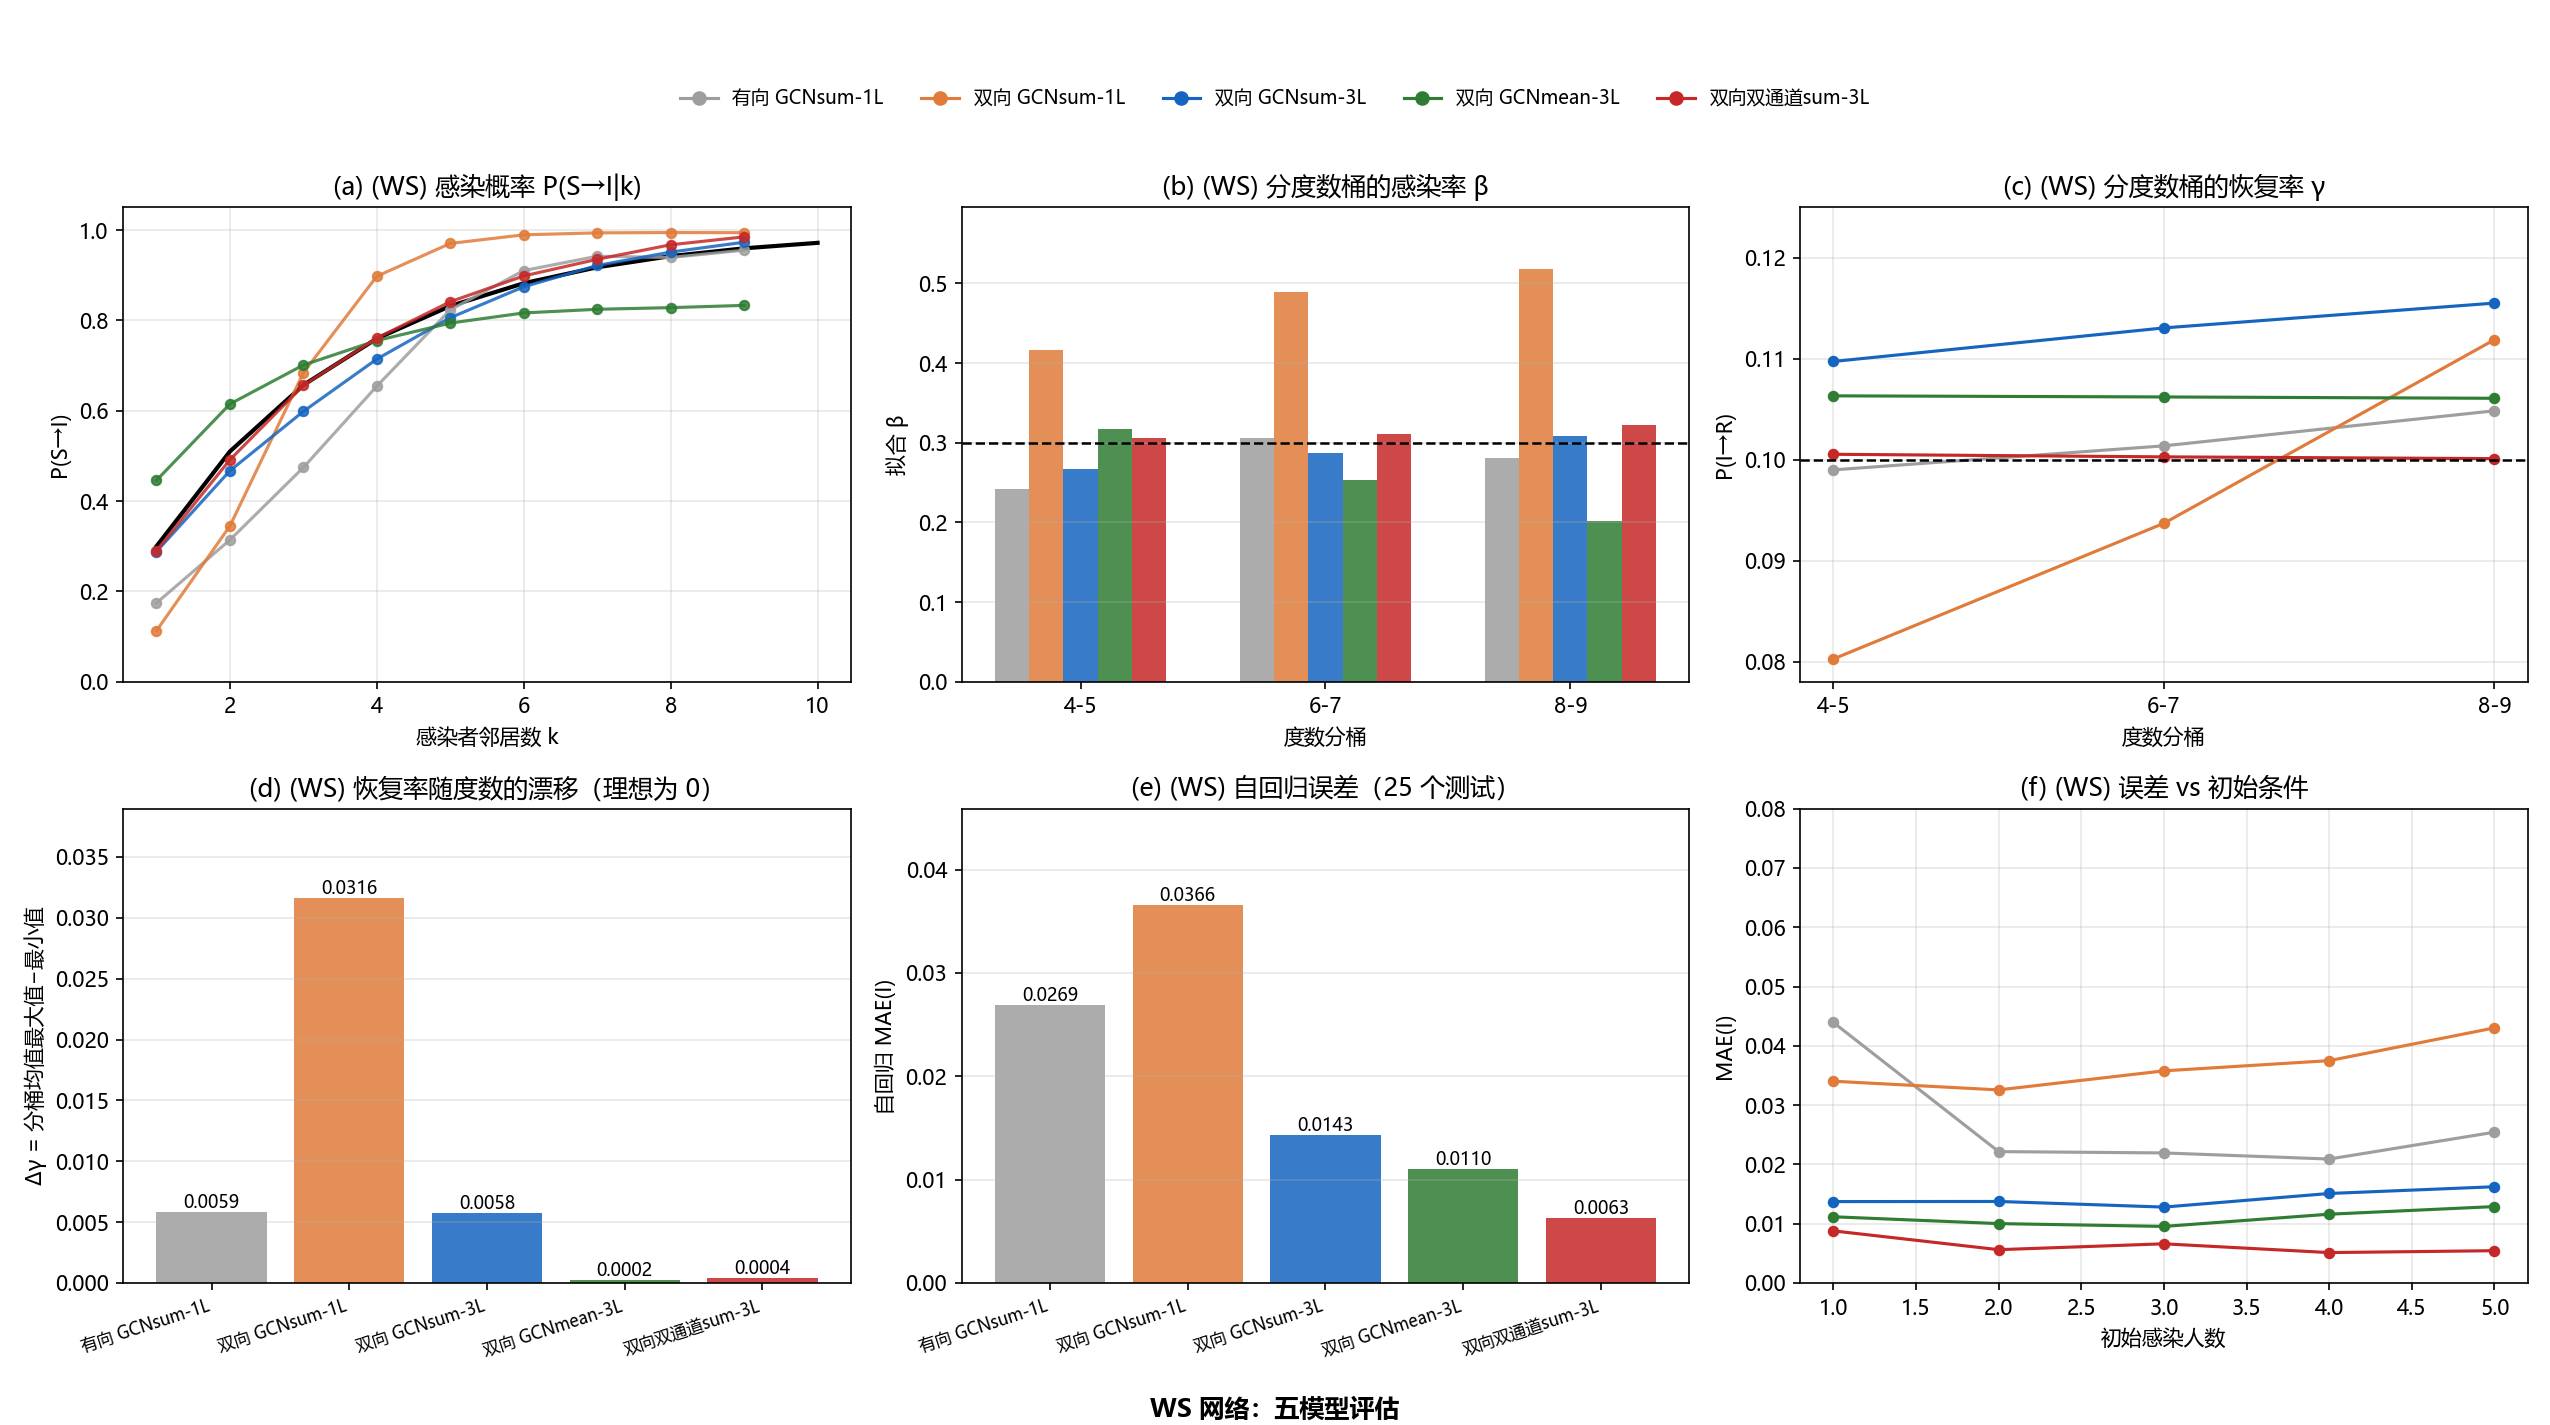
\includegraphics[width=0.96\linewidth]{fig_overview_WS.png}
  \caption{已知拓扑：WS 网络五模型完整诊断。}
\end{figure}
\end{landscape}

\begin{landscape}
\begin{figure}[p]
  \centering
  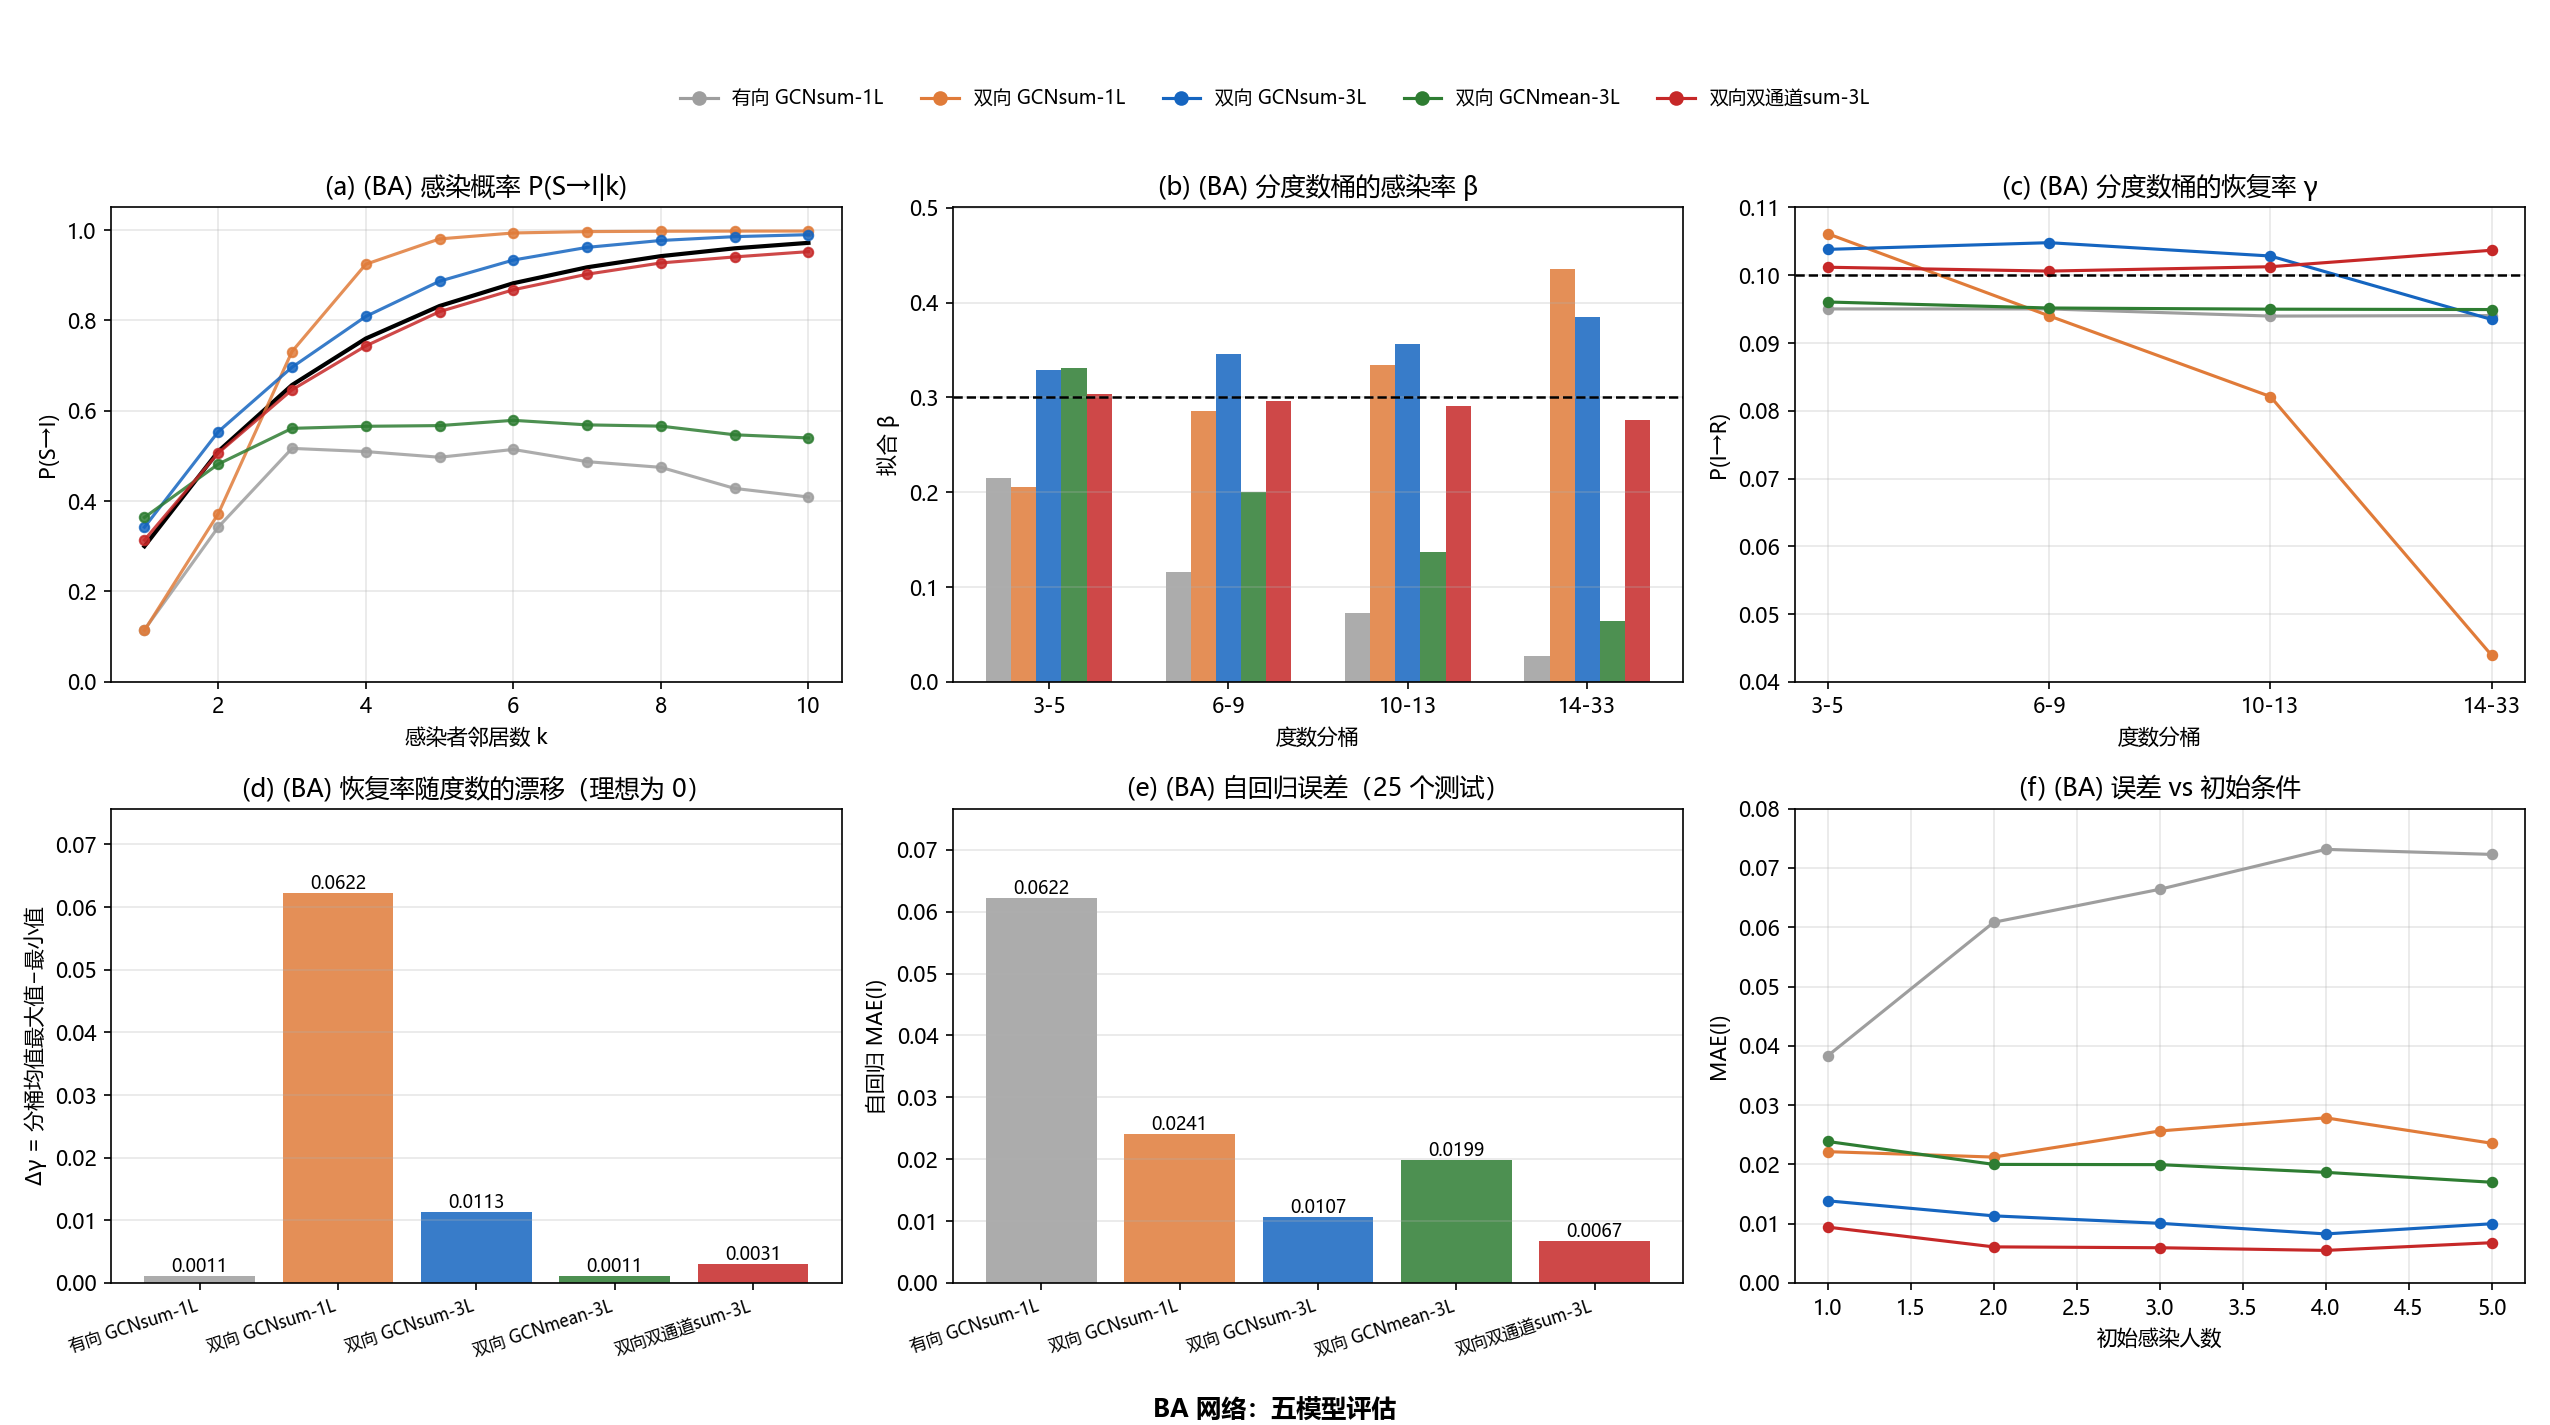
\includegraphics[width=0.96\linewidth]{fig_overview_BA.png}
  \caption{已知拓扑：BA 网络五模型完整诊断。}
\end{figure}
\end{landscape}

\subsection{未知拓扑完整诊断与训练曲线}

图\ref{fig:appendix-unknown-overview}给出未知拓扑所选模型的完整机制校准汇总，图\ref{fig:appendix-losses}给出三类网络的学习器损失、生成器损失、验证损失和温度轨迹。
训练曲线只能说明同分布状态对验证损失的变化，
不能据此判断轨迹级过拟合。

\begin{figure}[H]
  \centering
  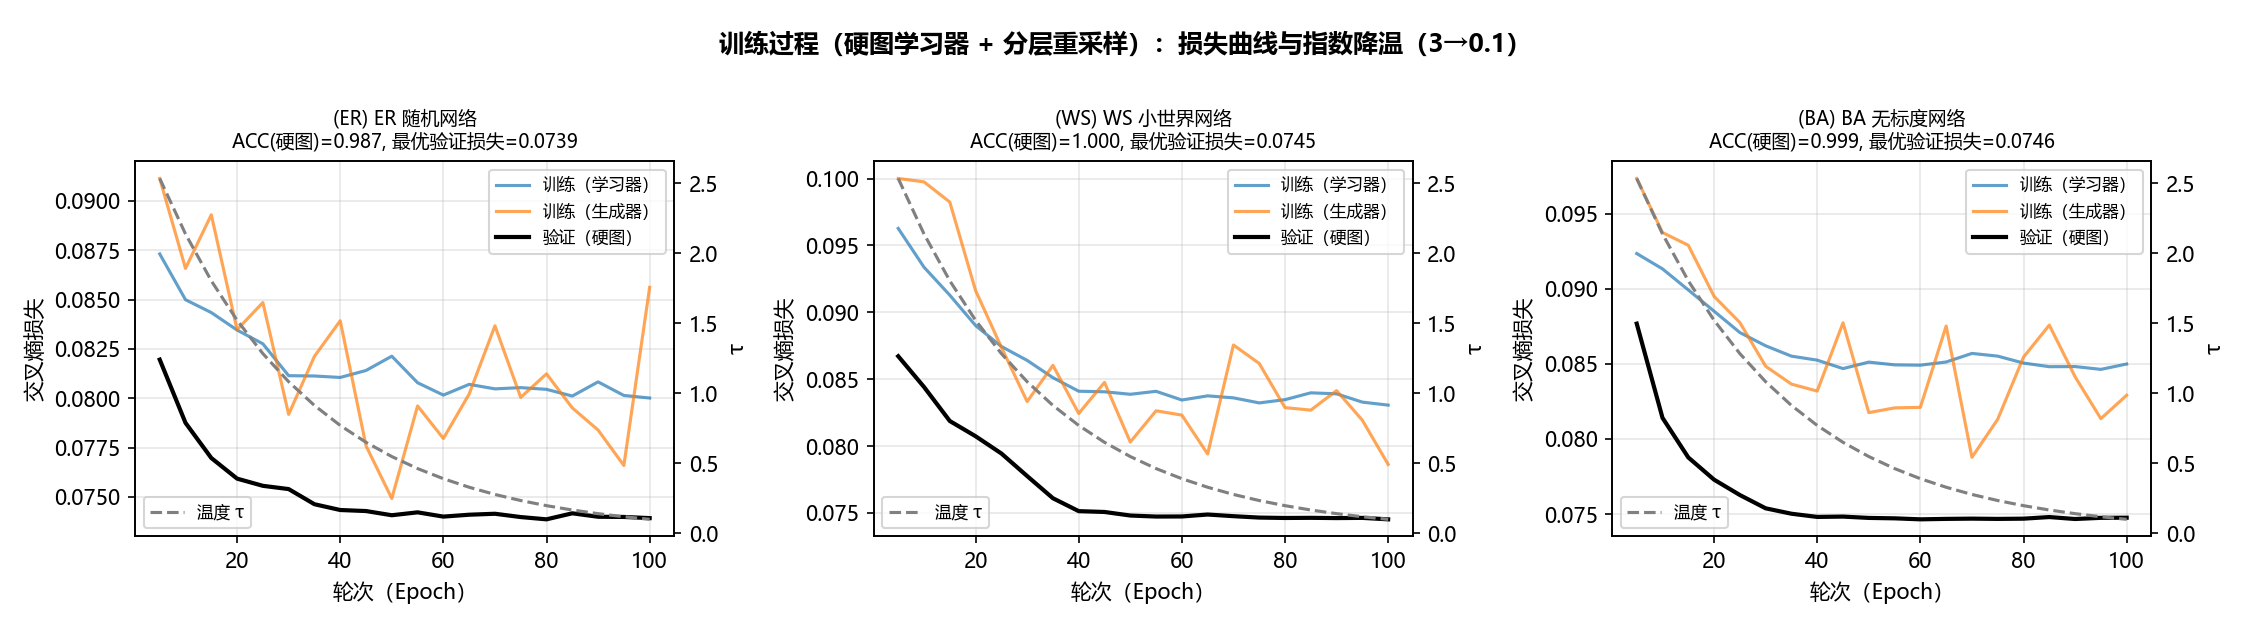
\includegraphics[width=\textwidth]{fig6_losses.png}
  \caption{未知拓扑：三个所选模型的训练损失、状态对级验证损失和温度变化。}
  \label{fig:appendix-losses}
\end{figure}

\begin{landscape}
\begin{figure}[p]
  \centering
  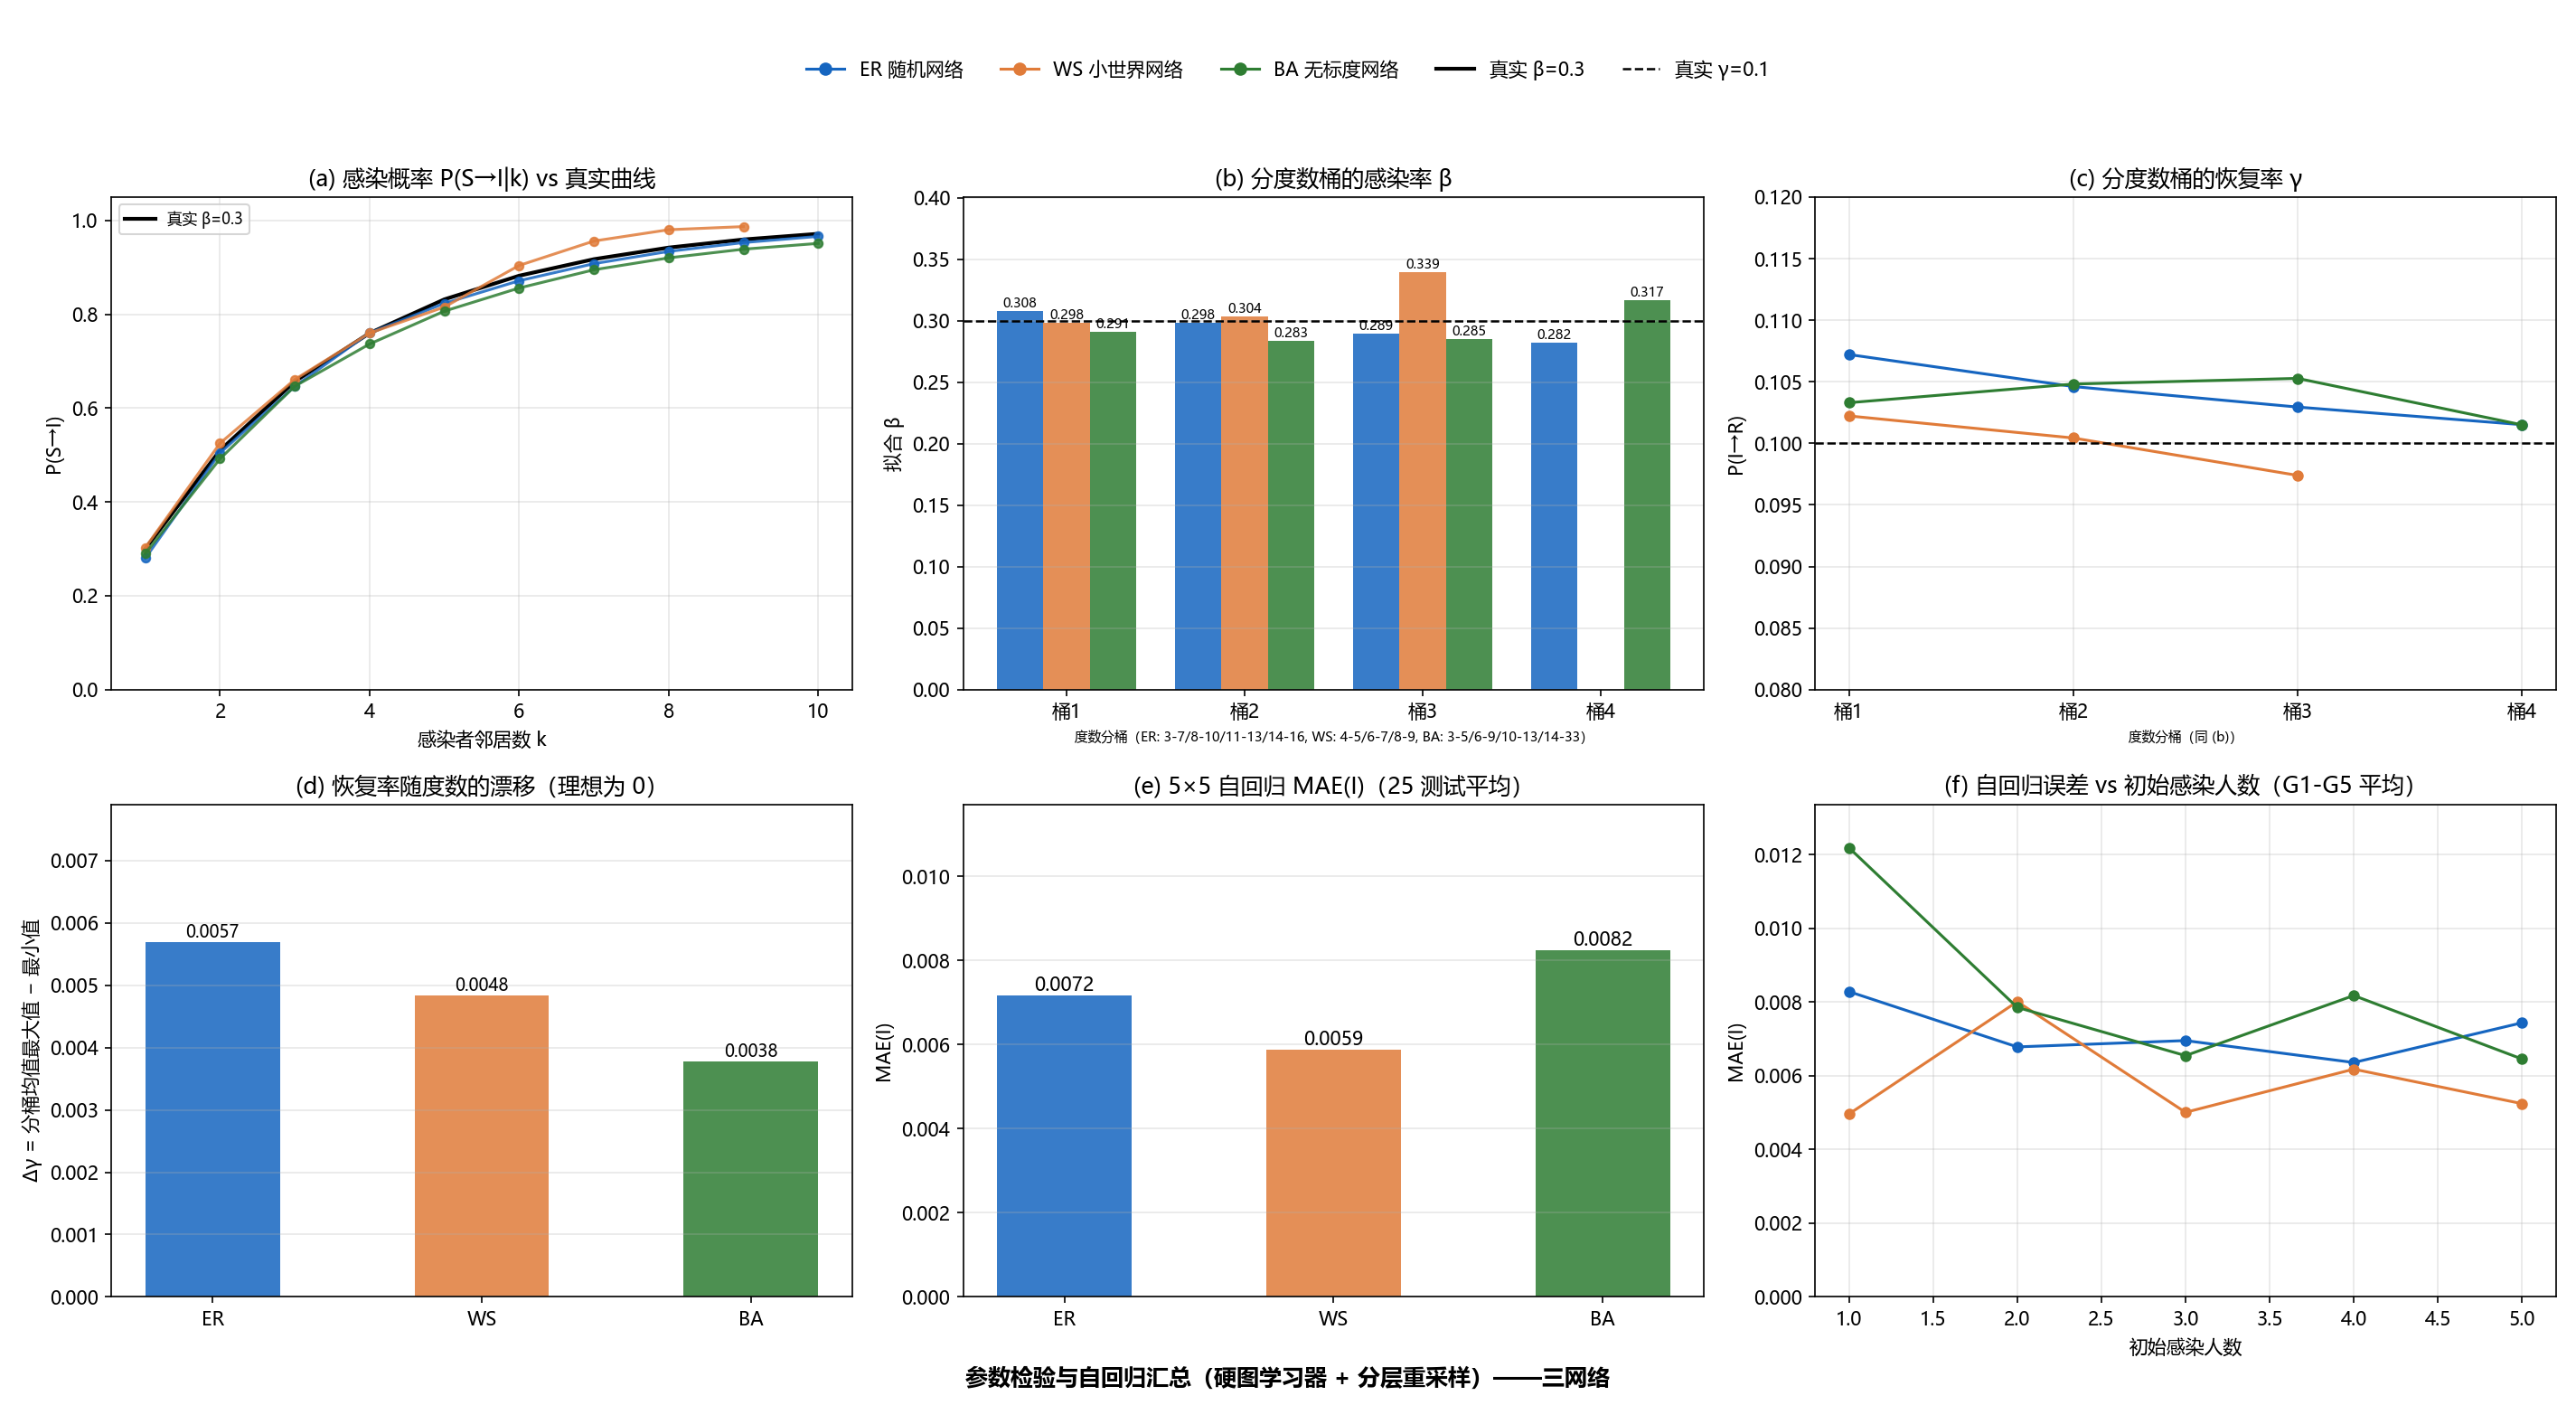
\includegraphics[width=0.96\linewidth]{fig6_overview_all.png}
  \caption{未知拓扑：所选 ER、WS、BA 模型的参数校准与自回归完整汇总。
正文数值从 JSON 重新读取，未直接从图中抄录。}
  \label{fig:appendix-unknown-overview}
\end{figure}
\end{landscape}

\clearpage
\subsection{完整 5×5 自回归网格}

图\ref{fig:appendix-autoreg-known-er}--图\ref{fig:appendix-autoreg-unknown-ba}保留所有自回归测试。
每张网格包含 5 组随机初始条件和 1--5 个初始感染者；
实线为真实模拟平均轨迹，
虚线为模型平均轨迹。
网格用于完整性核查，
正文只展示聚合误差和代表性平均曲线。

\begin{figure}[H]
  \centering
  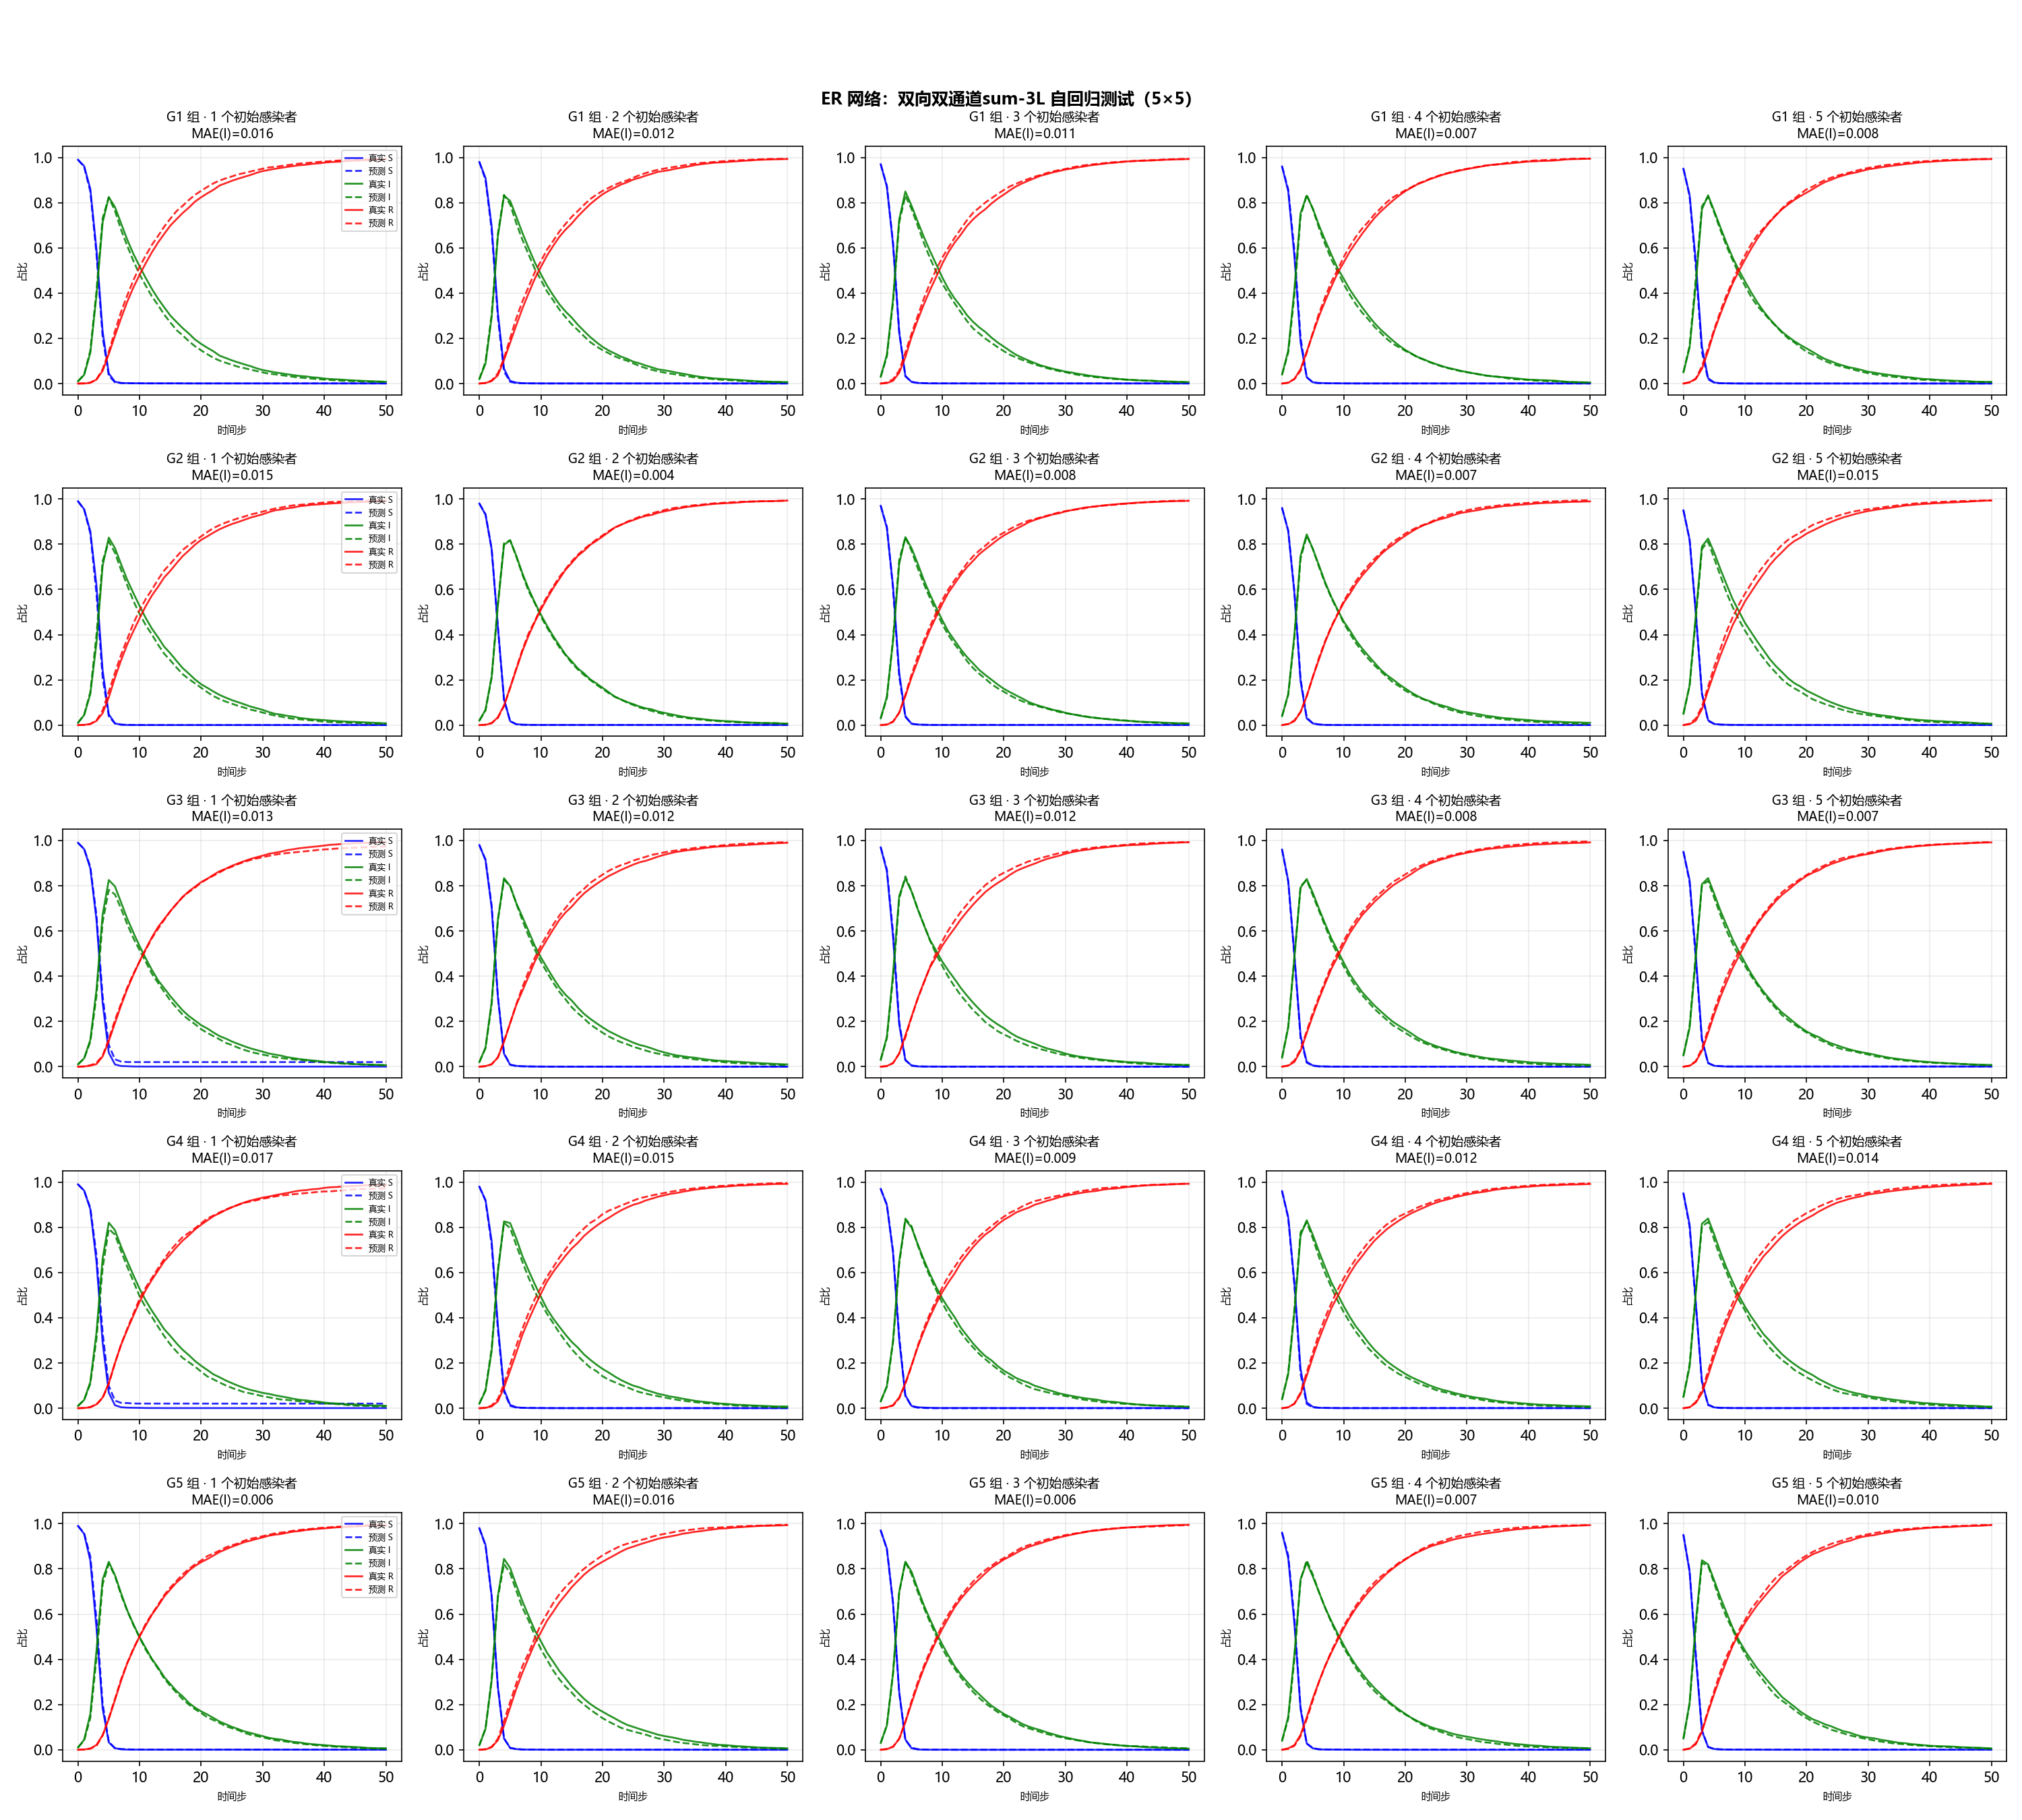
\includegraphics[width=0.95\textwidth]{fig_autoreg_grid_ER.png}
  \caption{已知拓扑双通道模型：ER 网络完整 5×5 自回归测试。}
  \label{fig:appendix-autoreg-known-er}
\end{figure}

\begin{landscape}
\begin{figure}[p]
  \centering
  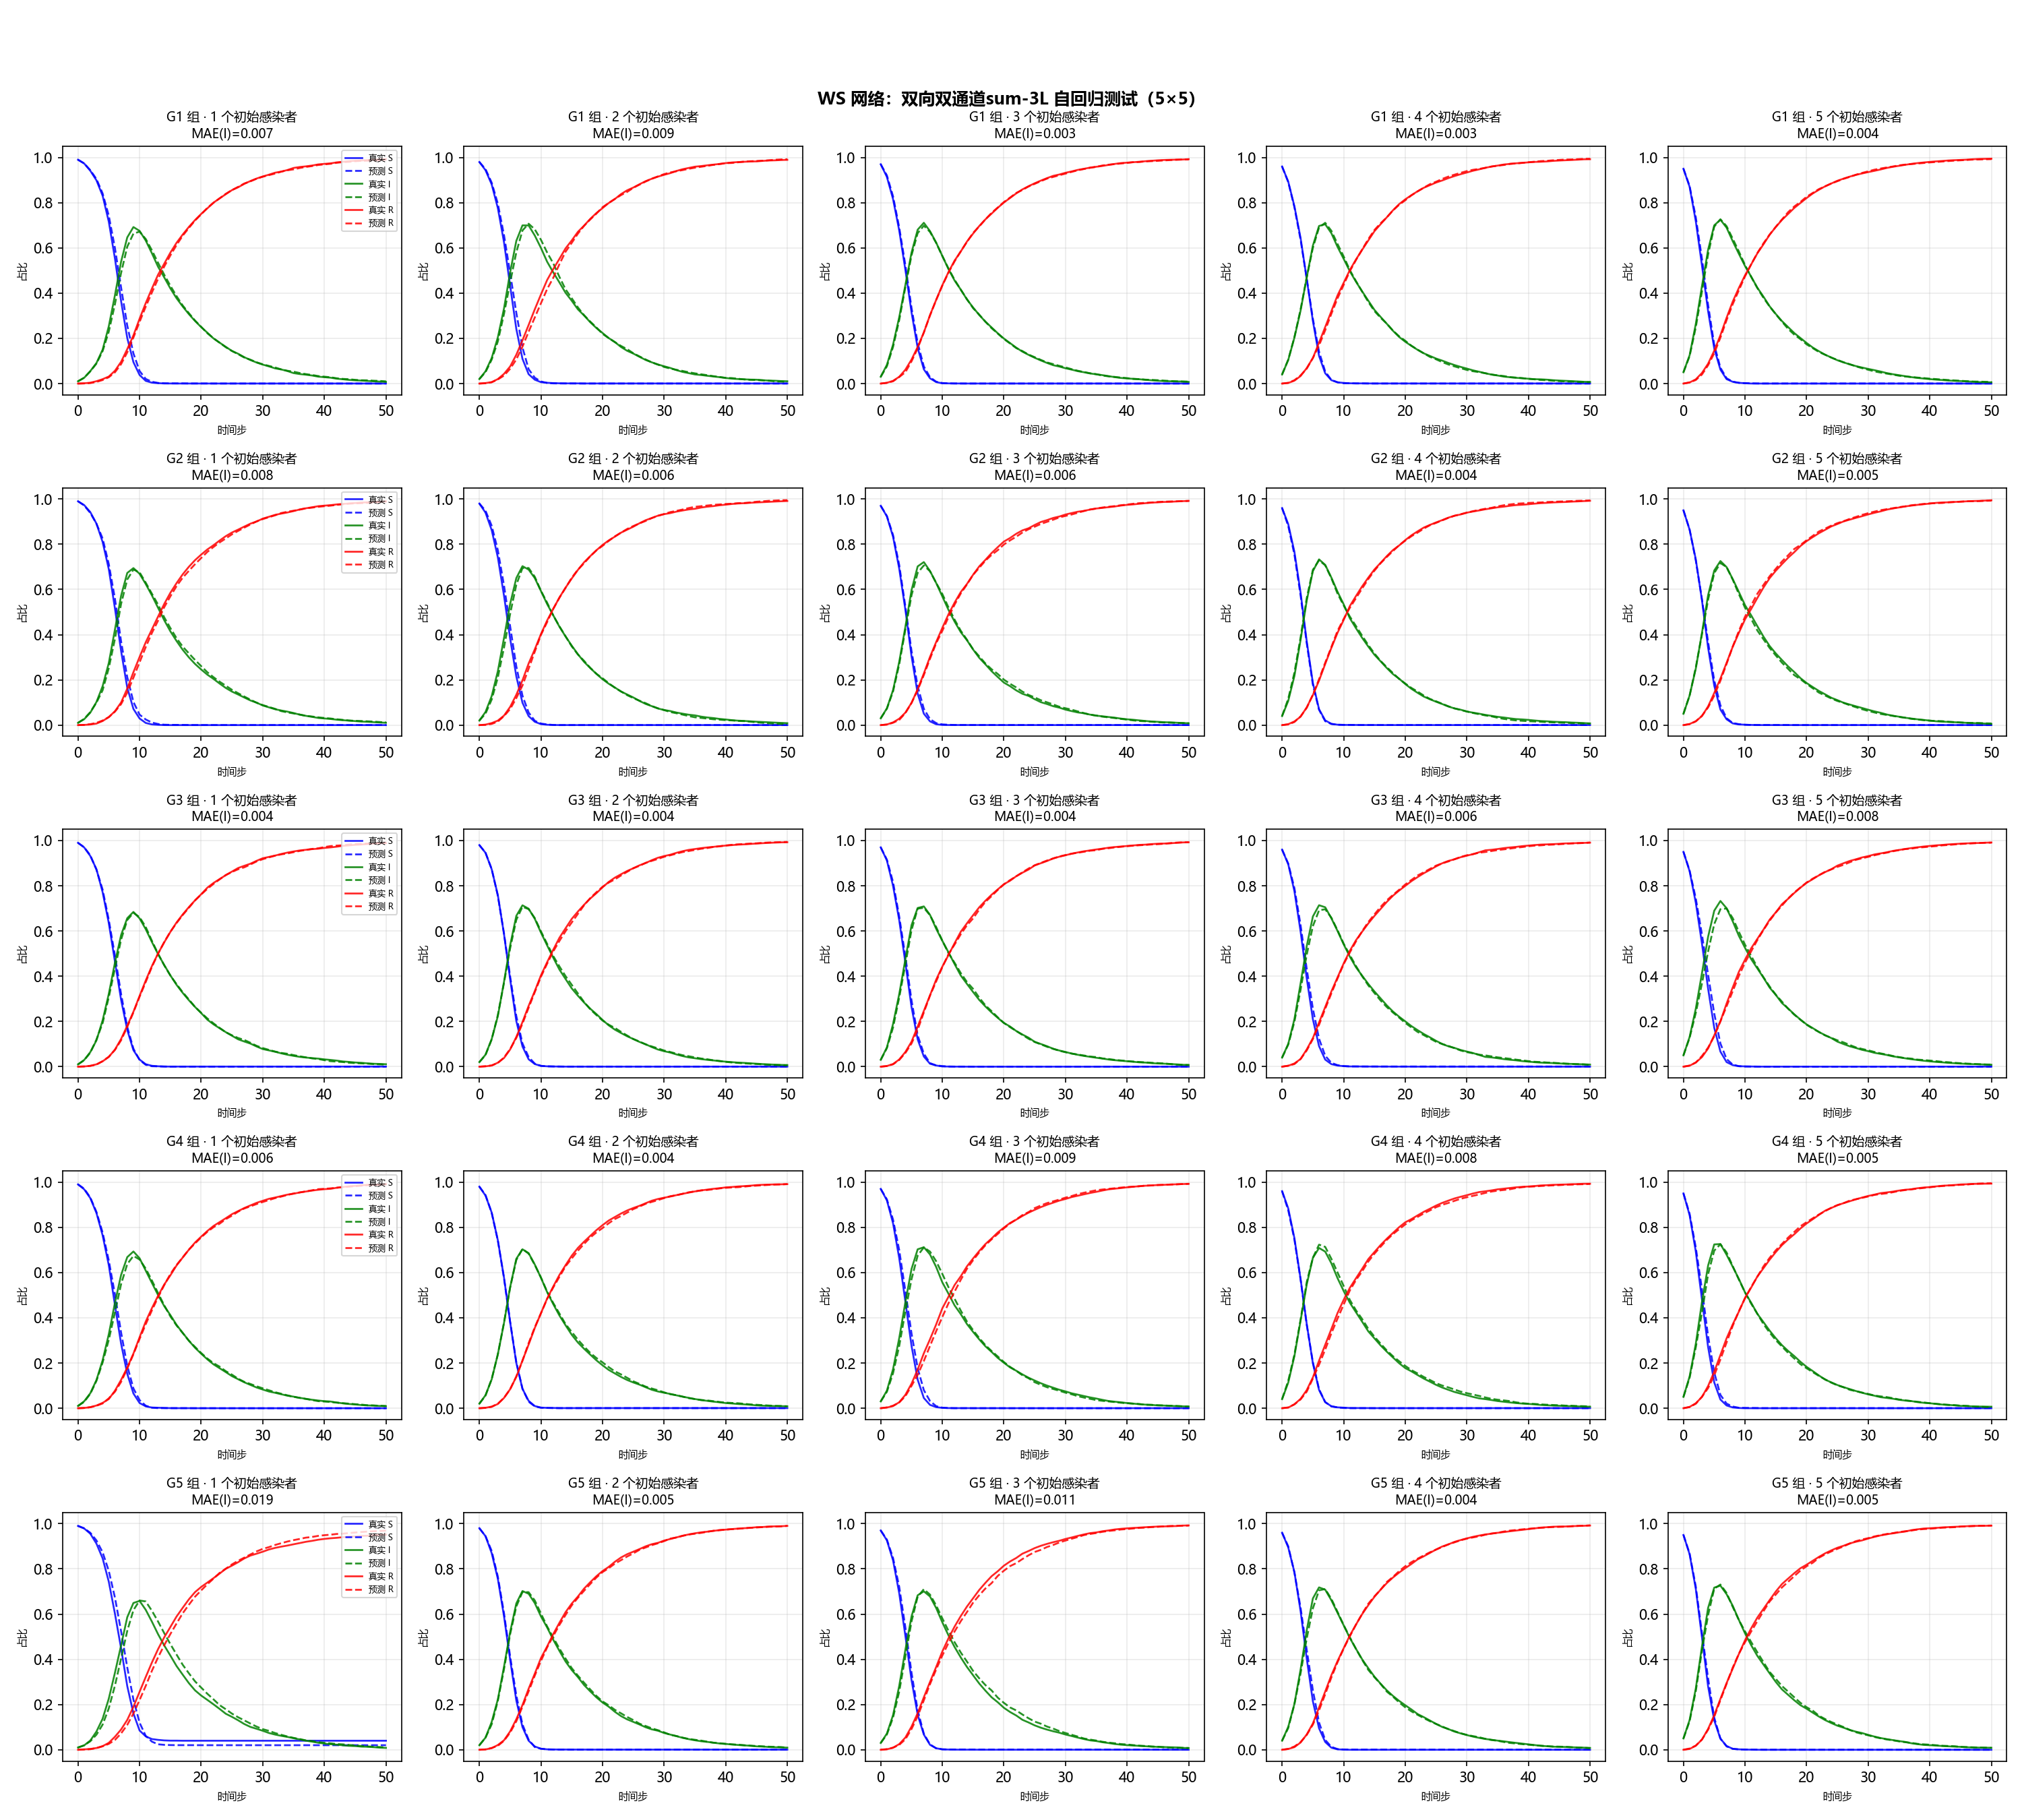
\includegraphics[height=0.86\textheight]{fig_autoreg_grid_WS.png}
  \caption{已知拓扑双通道模型：WS 网络完整 5×5 自回归测试。}
\end{figure}
\end{landscape}

\begin{landscape}
\begin{figure}[p]
  \centering
  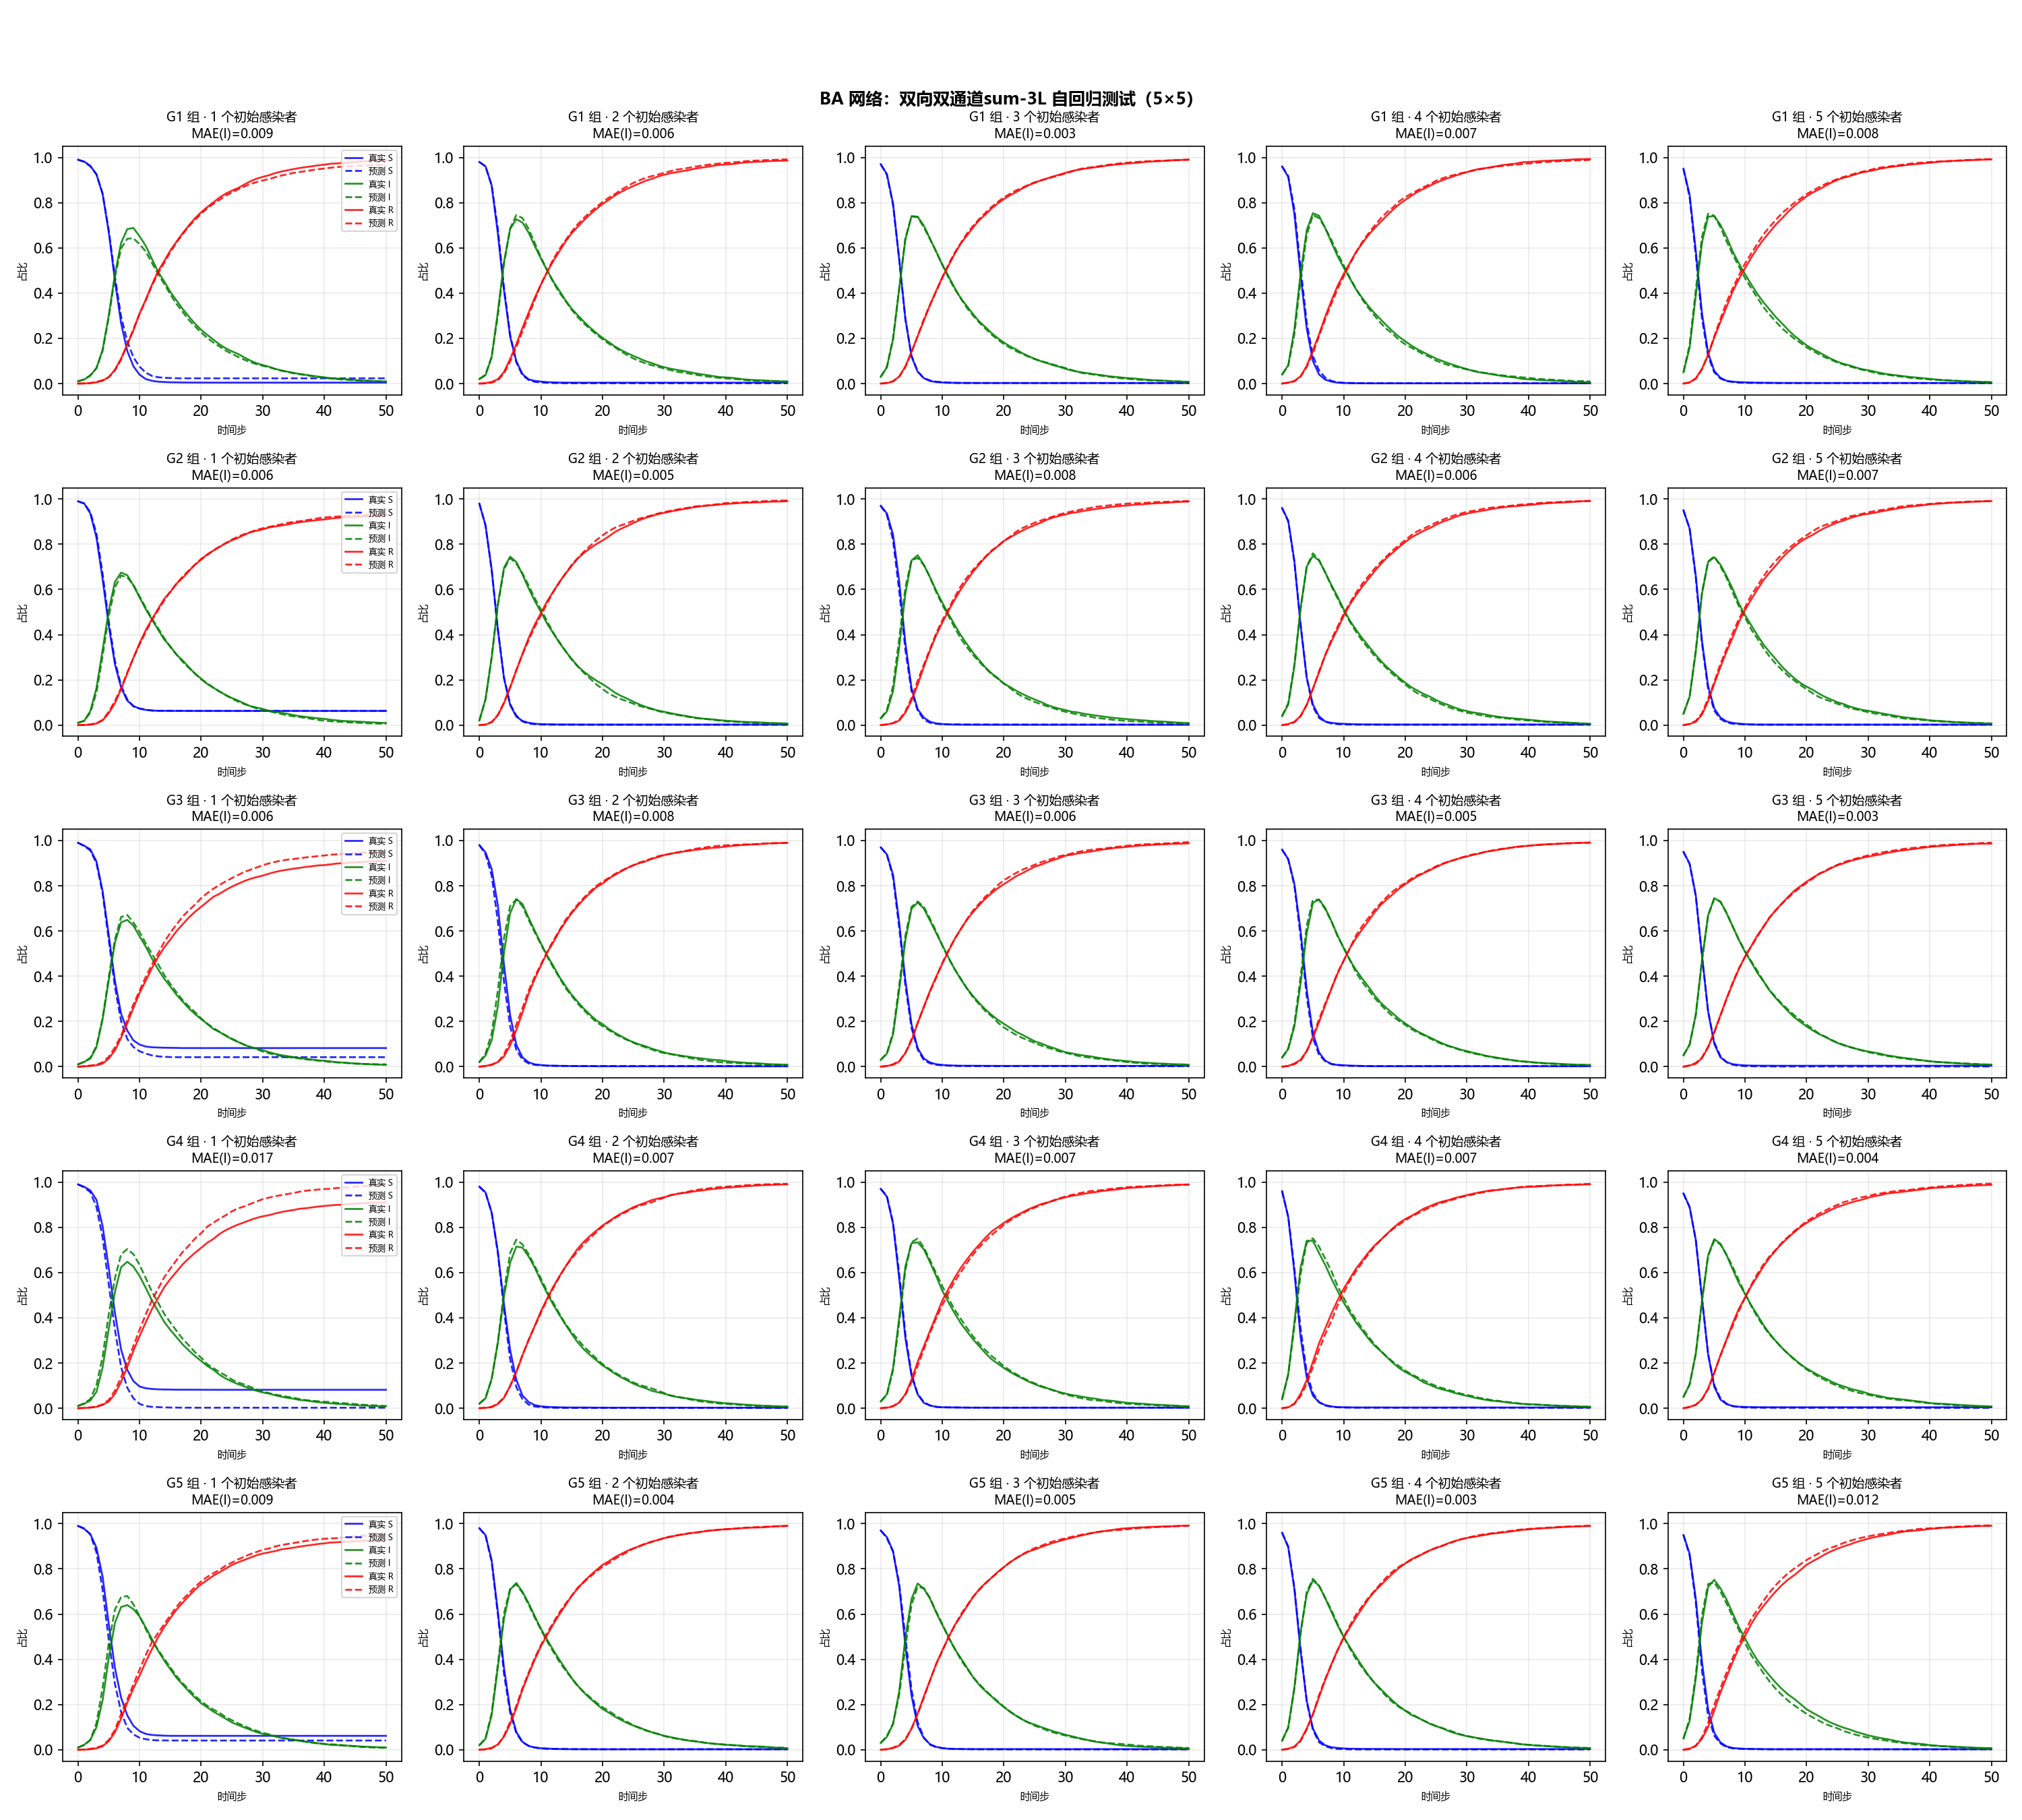
\includegraphics[height=0.86\textheight]{fig_autoreg_grid_BA.png}
  \caption{已知拓扑双通道模型：BA 网络完整 5×5 自回归测试。}
\end{figure}
\end{landscape}

\begin{landscape}
\begin{figure}[p]
  \centering
  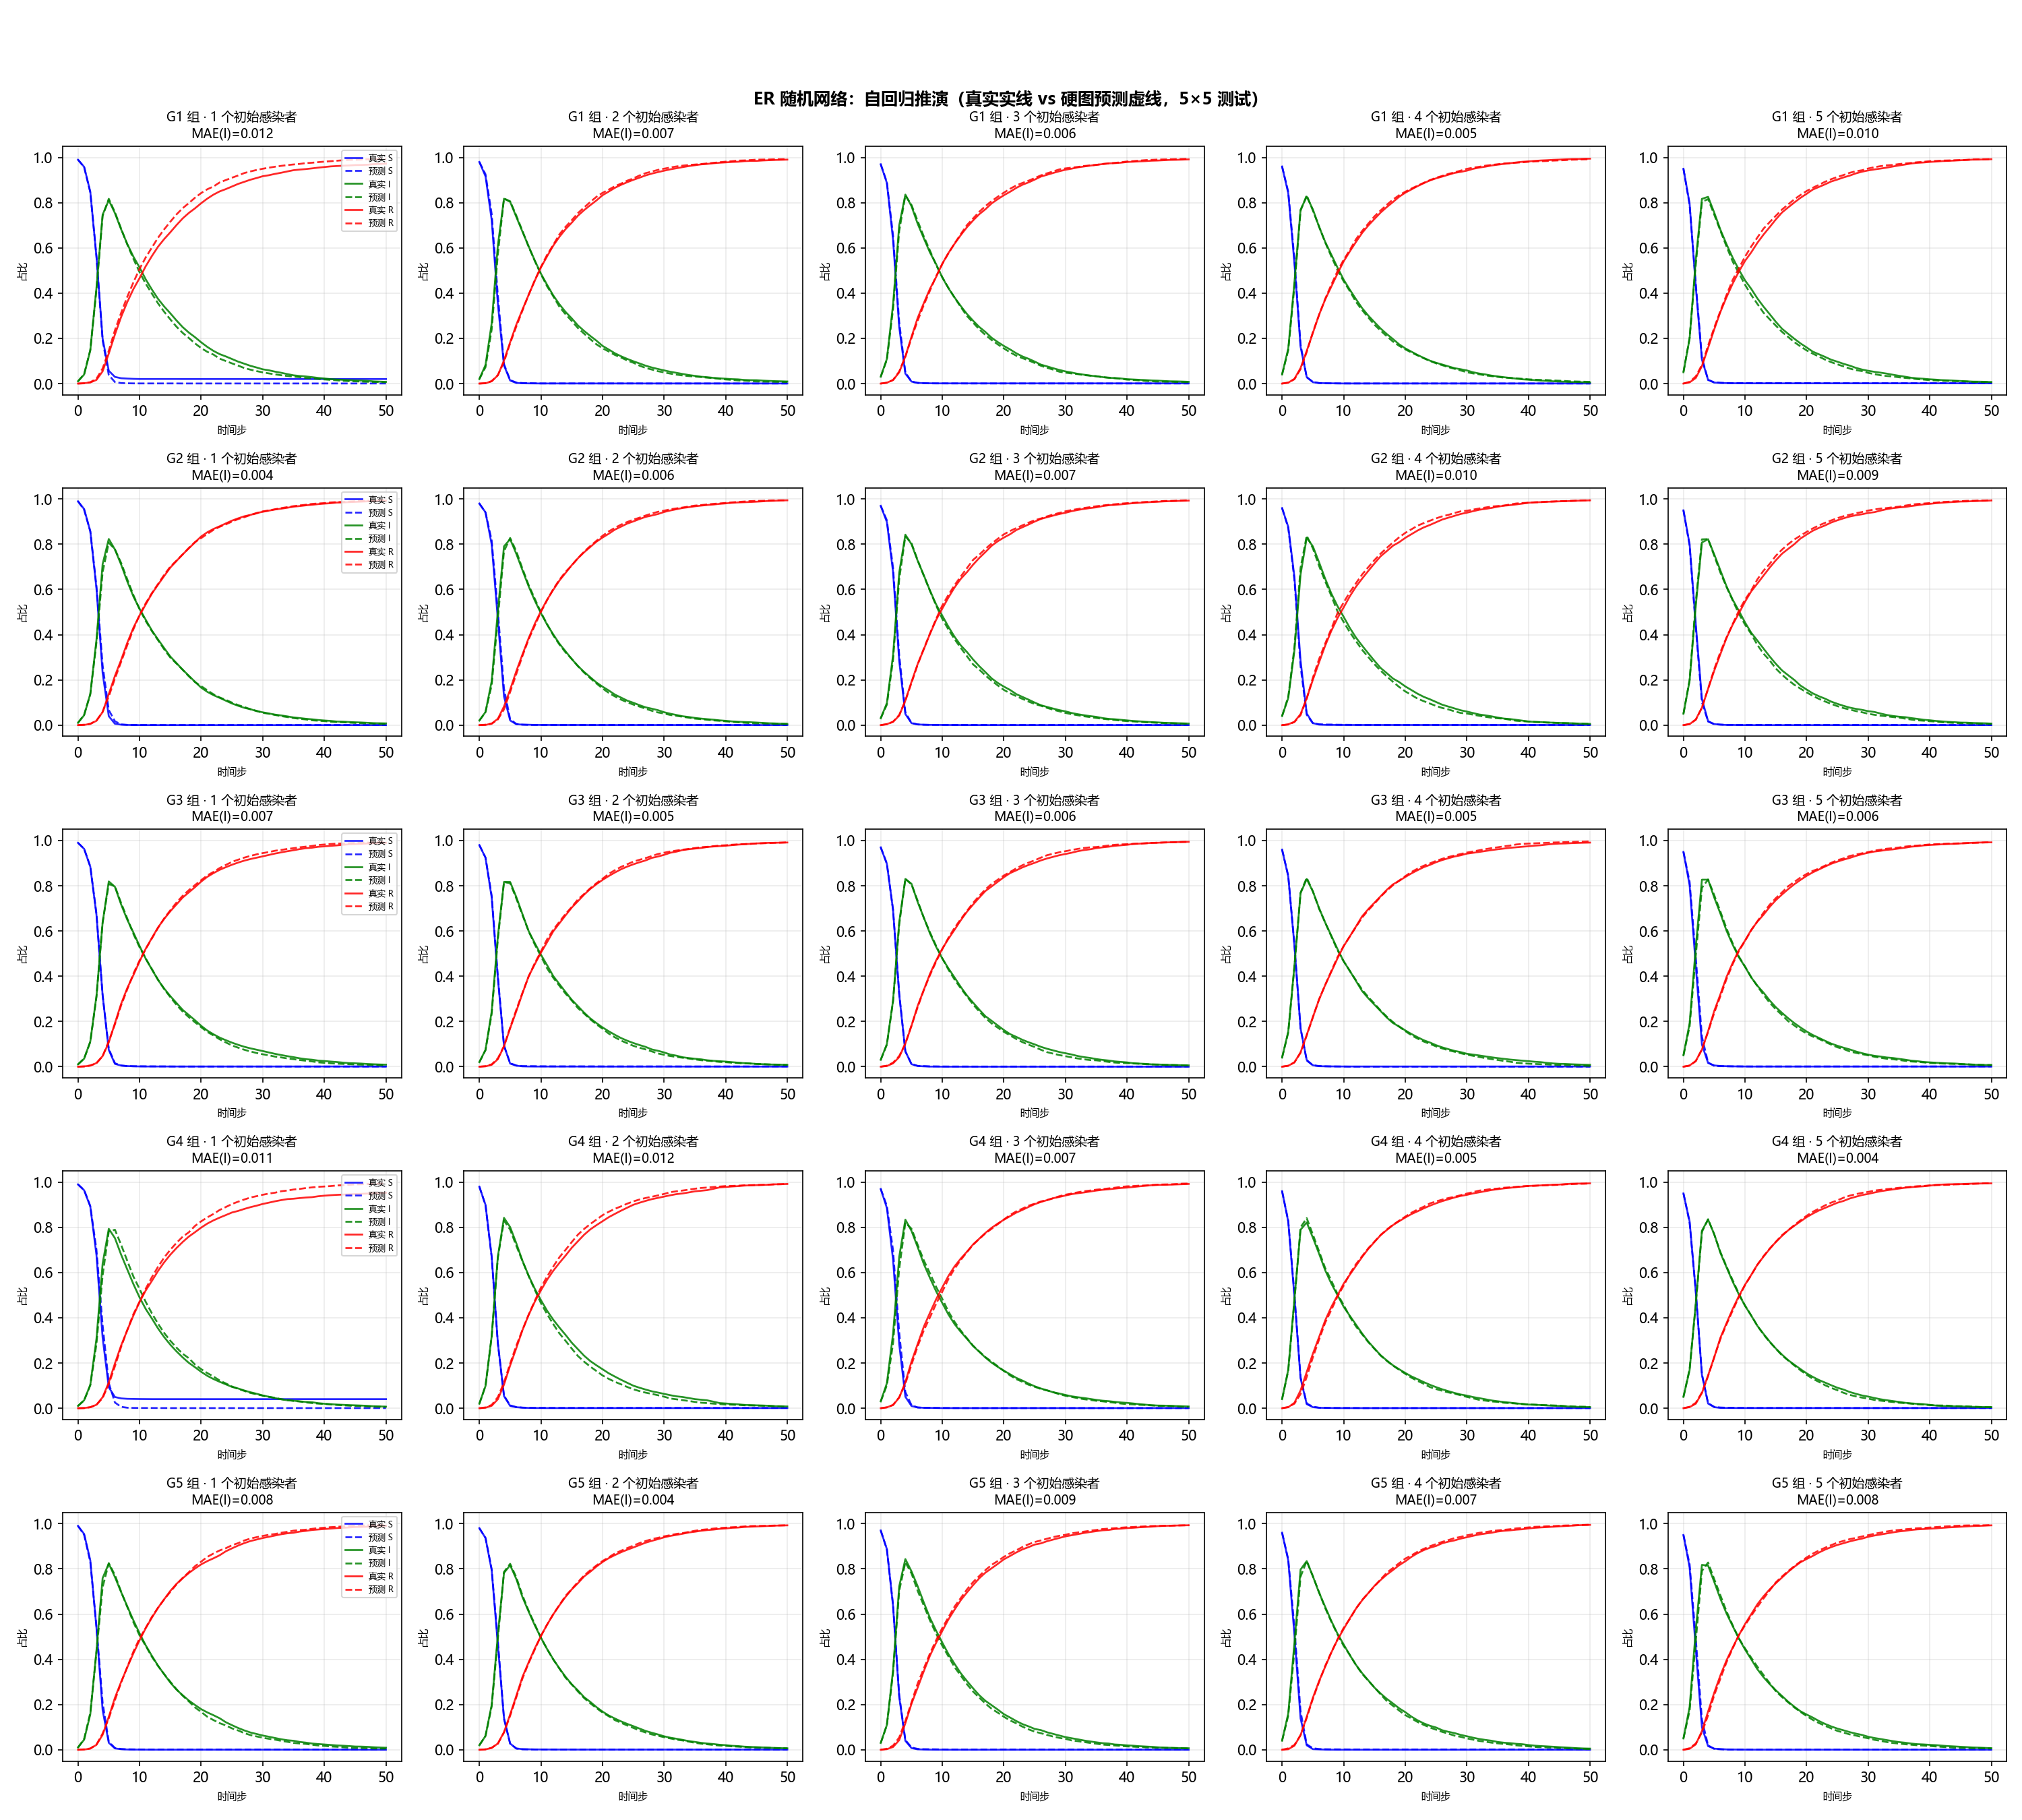
\includegraphics[height=0.86\textheight]{fig6_autoreg_grid_ER.png}
  \caption{未知拓扑所选模型：ER 网络完整 5×5 自回归测试。}
\end{figure}
\end{landscape}

\begin{landscape}
\begin{figure}[p]
  \centering
  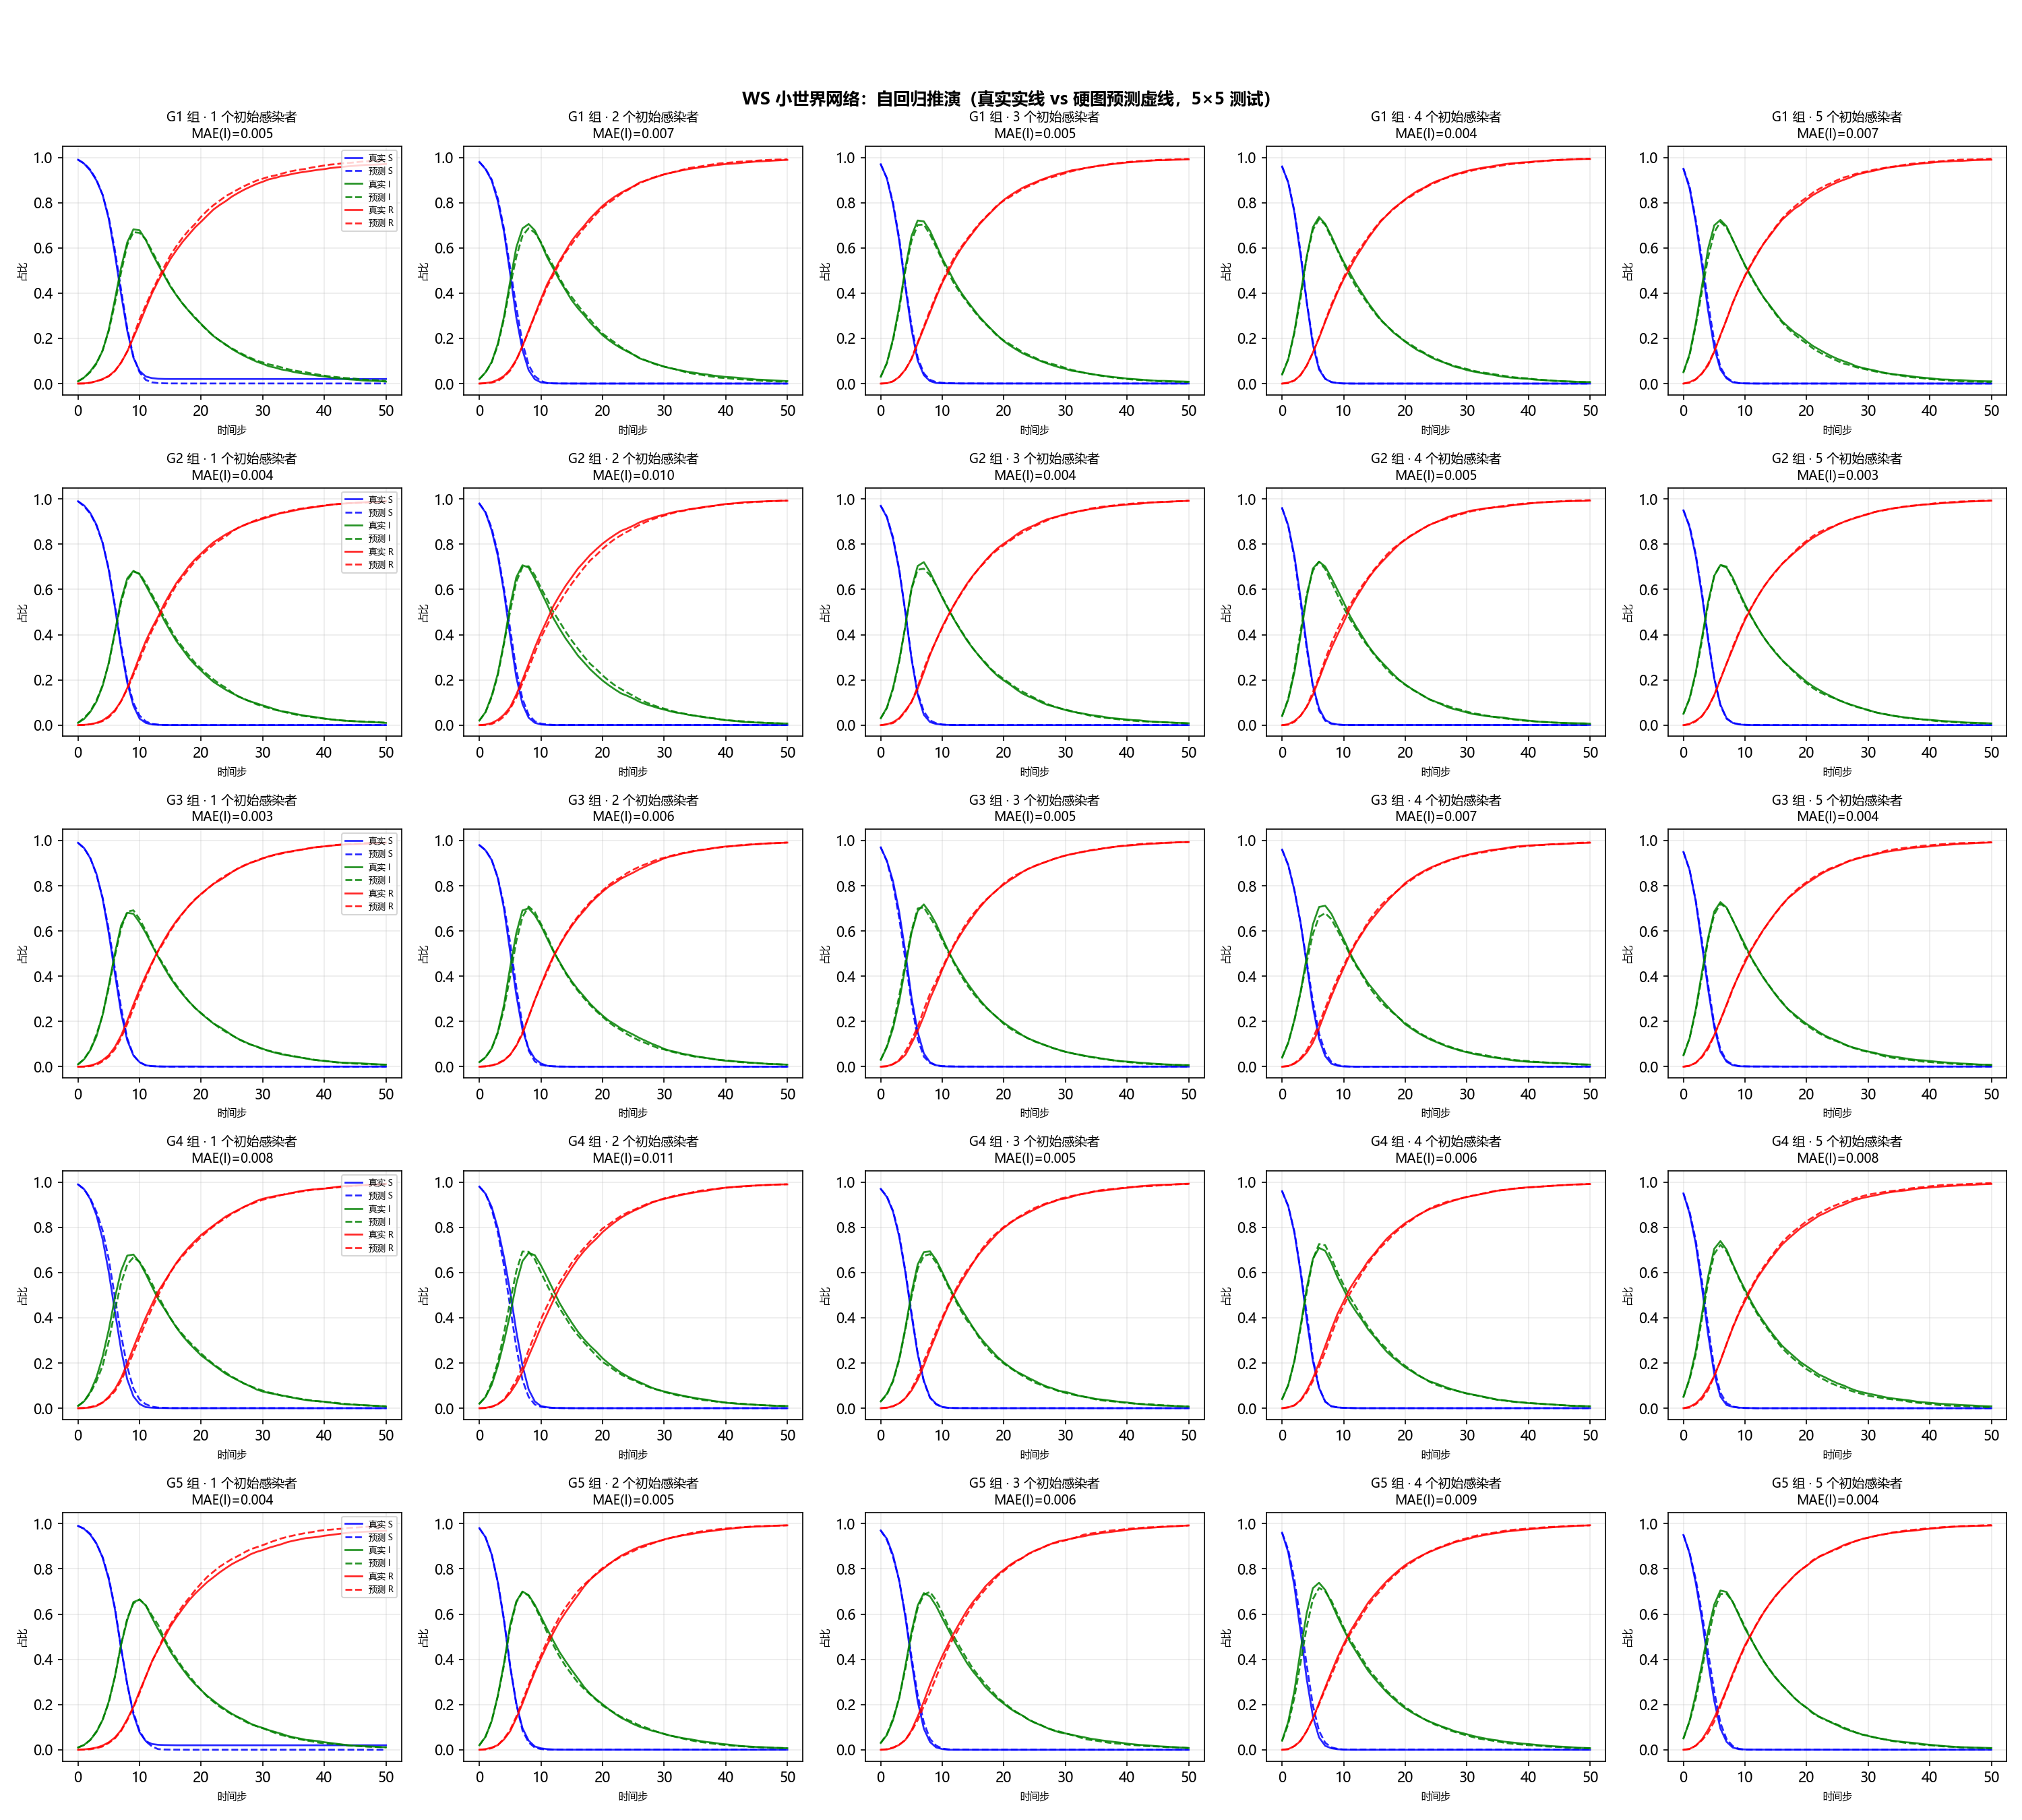
\includegraphics[height=0.86\textheight]{fig6_autoreg_grid_WS.png}
  \caption{未知拓扑所选模型：WS 网络完整 5×5 自回归测试。}
\end{figure}
\end{landscape}

\begin{landscape}
\begin{figure}[p]
  \centering
  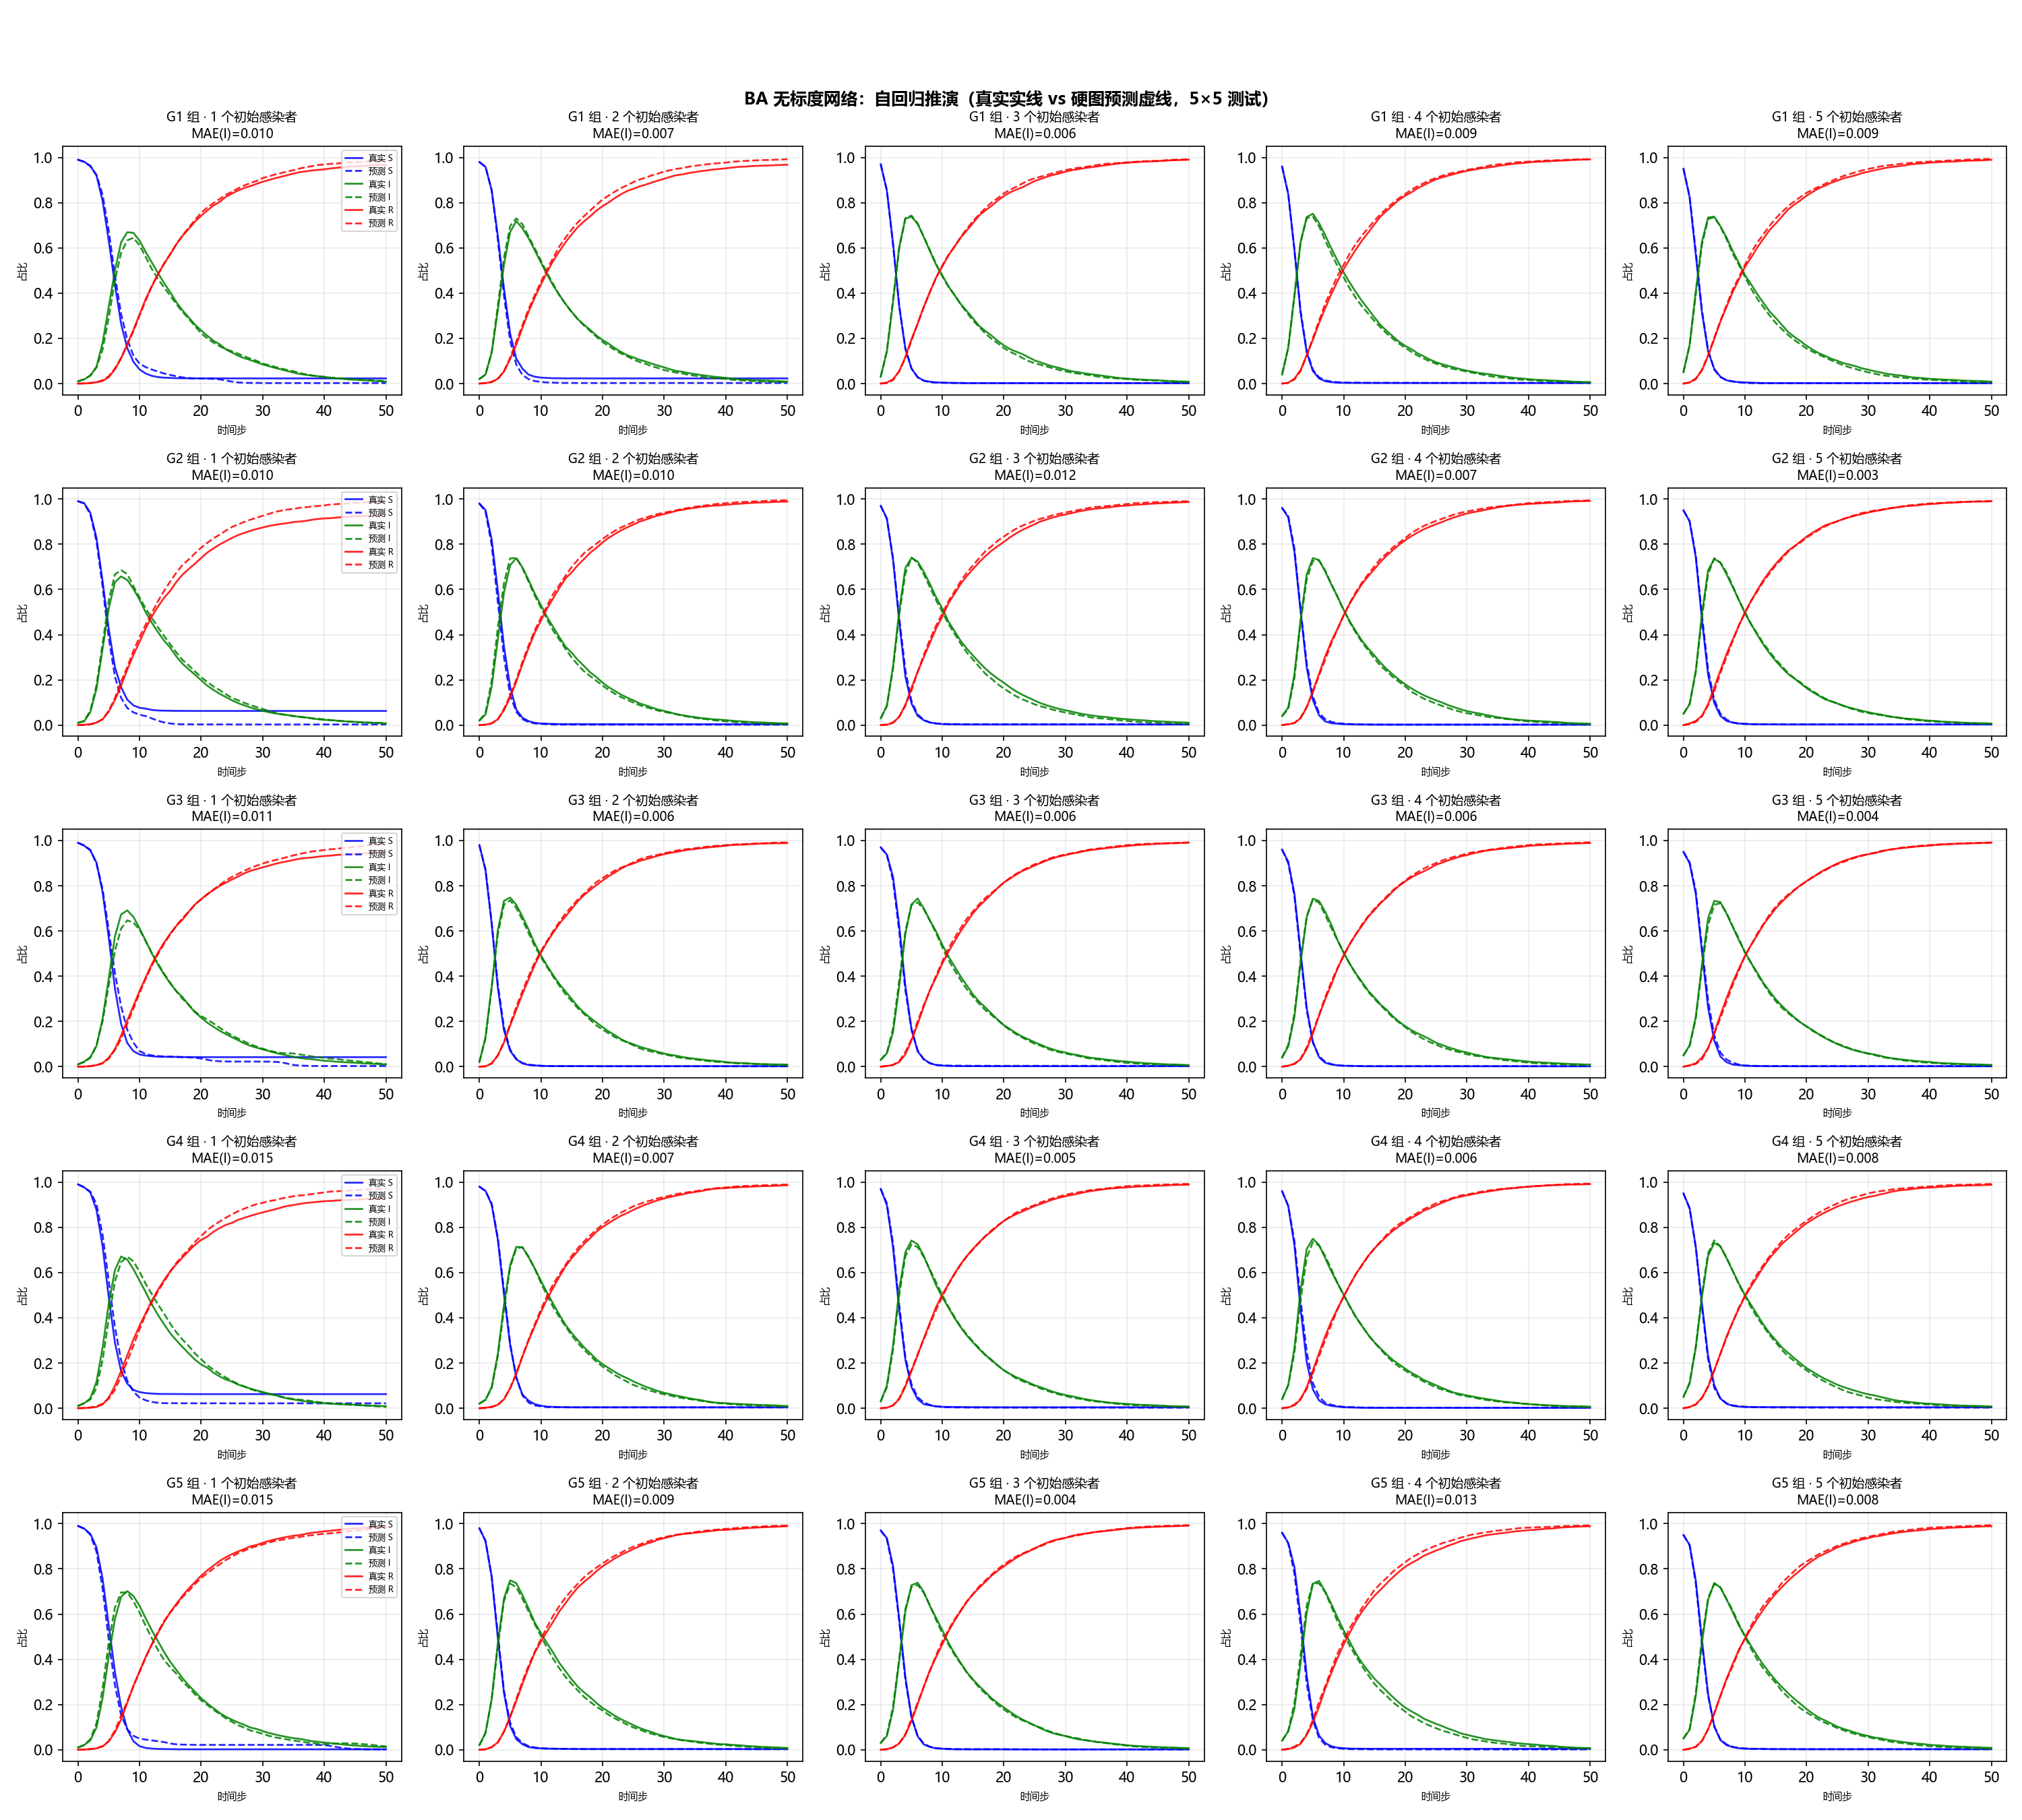
\includegraphics[height=0.86\textheight]{fig6_autoreg_grid_BA.png}
  \caption{未知拓扑所选模型：BA 网络完整 5×5 自回归测试。}
  \label{fig:appendix-autoreg-unknown-ba}
\end{figure}
\end{landscape}

\clearpage
\subsection{探索性失败实验汇总}

表\ref{tab:negative-results}汇总能够从保存 JSON 直接追溯的主要负结果。
不同配置之间不满足严格单变量条件，
因此这些数字只说明“在相应 BA 实例与配置下未改善”，
而不支持普遍方法定律。

\begin{table}[H]
  \centering
  \caption{未知拓扑开发阶段的探索性结果。}
  \label{tab:negative-results}
  \begin{tabularx}{0.92\textwidth}{@{}lXr@{}}
    \toprule
    网络/方案 & 说明 & 硬图 ACC \\
    \midrule
    ER 基础硬图版 & phase6 basic & 0.908 \\
    WS 基础硬图版 & phase6 basic & 0.998 \\
    BA 基础硬图版 & phase6 basic & 0.818 \\
    BA 两阶段版 & 软图粗学后硬图精修 & 0.888 \\
    BA 闭环多步 $P=2$ & 离散状态闭环回馈 & 0.562 \\
    BA 闭环多步 $P=3$ & 离散状态闭环回馈 & 0.299 \\
    BA teacher-forcing $P=2$ & 真实中间状态回馈 & 0.578 \\
    BA teacher-forcing $P=3$ & 真实中间状态回馈 & 0.496 \\
    \bottomrule
  \end{tabularx}
\end{table}

\section{复现文件与软件环境}

\subsection{来源文件}

正文数值的唯一实验来源如下：
\begin{itemize}
  \item \nolinkurl{two_channel_experiment/results/phase4/phase4_five_models.json}；
  \item \nolinkurl{two_channel_experiment/results/phase6/dgsl_l1b_ER.json}、\nolinkurl{WS.json}、\nolinkurl{BA.json}；
  \item phase6 中 ER/WS/BA 各 seed 7、21、42 的九个逐 seed JSON。
\end{itemize}
\nolinkurl{paper/notebooks/} 中的两份 notebook 分别生成三张方法图和三张结果图，
并由结果绘图 notebook 生成 \nolinkurl{metrics_manifest.json}。
\nolinkurl{paper/scripts/build_figures.py} 为统一执行入口。
清单包含全部来源 SHA-256、派生 Precision/F1、跨网络平均指标及选中模型。
\nolinkurl{paper/scripts/verify_results.py} 再次核对哈希、phase4 关键数值、最低验证 CE 选模规则和 phase6 边数。

\subsection{软件版本}

实验环境经实际虚拟环境核对为：Python 3.13.7、PyTorch 2.12.0+cpu\cite{paszke2019}、PyTorch Geometric 2.7.0\cite{fey2019}、NetworkX 3.5\cite{hagberg2008}、NumPy 2.2.6、SciPy 1.16.2、Matplotlib 3.10.6，
优化器使用 Adam\cite{kingma2015adam}。
未知拓扑实现参考 GGN 官方代码的交替训练语义\cite{ggncode}。
论文使用 TeX Live 2025、XeLaTeX、latexmk 4.87 和 biber 2.21 编译；
PDF 使用 Poppler 26.07 渲染检查。

\subsection{结果解释约定}

为避免常见误读，复现时采用以下约定：
\begin{enumerate}
  \item “5×5”指 5 组评估初始条件与 1--5 个初始感染者，不是 5 个训练 seed；
  \item $\hat\gamma\pm s$ 中的 $s$ 是控制状态上的输出离散度，不是置信区间；
  \item phase4 的最终结果已使用修复后的 SIR 邻接去重模拟器；
phase0/phase1 的旧自回归数值不纳入正文；
  \item 未知拓扑的 data seed 固定为 21，train seed 为 7、21、42；
训练 seed 的变化不得触发重新生成真实图；
  \item 若修改网络、$\beta$、$\gamma$ 或 $T$，必须同时更新缓存键或删除旧缓存，不能无条件复用 \code{data\_ER.npz} 等文件。
\end{enumerate}


\end{document}
